\pagenumbering{arabic}
%\documentclass[slides]{beamer}
\documentclass[mathserif, 10pt]{beamer}
\usepackage[framesassubsections]{beamerprosper}
\setbeamercovered{transparent}
%\documentclass[slides,hyperref={pdfpagelabels=false}]{beamer}
%\documentclass[handout,gray]{beamer}
\usepackage[T1]{fontenc}
\usepackage[utf8]{inputenc}
\usepackage{textcomp}
\usepackage{algorithm}
\usepackage{algorithmic}
\usepackage{color}
\usepackage{braket}
\usepackage{verbatim}
\usepackage{amsbsy}
\usepackage{multirow}
\usepackage{multicol}
\usepackage{booktabs} % Make some nice tables
\usepackage{ae,aecompl}

%%%%%%%%%%%% COULEURS %%%%%%%%%%%%%%%%%%%%%%%%%%%

\mode<presentation>
{
  \definecolor{beamerstructure}{RGB}{43,79,112}
  \definecolor{sidebackground}{RGB}{230,242,250}
  \definecolor{CTCC}{RGB}{133,188,228}
  \color{beamerstructure}
  \usetheme{default}
  \usepackage{courier}
  \beamertemplateballitem
\setbeamertemplate{navigation symbols}{}
%\setbeamertemplate{sidebar left}{\thispdfpagelabel{\insertframenumber}}
%\setbeamertemplate{footline}{\quad\insertframenumber}
%\usecolortheme{CTCC}
}
\usebackgroundtemplate{
\includegraphics[width=1.02\paperwidth] {figures/ctcc_general.jpg}}

\title{\\\vspace{1cm}
Magnetic properties with multiwavelets
}
%\subtitle{\textcolor{magenta}{My subtitle (if applicable)}}
\author{Stig Rune Jensen}
\institute[CTCC]{\\[-6mm]stig.r.jensen@uit.no\\
[6mm]UiT - The Arctic University of Norway\\[6mm]

\includegraphics[height=1.5cm]{figures/uio.pdf}\hspace{1cm} 

\includegraphics[height=1.5cm]{figures/sff.pdf}\hspace{1cm}

\includegraphics[height=1.5cm]{figures/uit.pdf}}
\date{Stony Brook, 4 August 2016}

%\newtheorem{lemma}{Proposition}
\newcommand{\fixme}[1]{{\small\em \color{red} #1 \normalsize}}

\newcommand{\unitboxd}{\ensuremath{\left[0,1\right]^d}}
\newcommand{\Exp}[1]  {\ensuremath{\cdot 10^{#1}}}
\newcommand{\etal}{{\emph{et al.}\ }}
\newcommand{\abinitio}{{\emph{ab initio }\ }}
\newcommand{\mycomment}[1]{{\large \bf #1}}
\newlength{\dch}
\newlength{\sch}
\newcommand{\ud}{\ensuremath{\,\mathrm{d}}}
\newcommand{\mydef}{\stackrel{\text{def}}{\hbox{=}}}
\newcommand{\setdch}{\settoheight{\dch}{\nscu{d}}}
\newcommand{\setsch}{\settoheight{\sch}{\nscucd{s}}}
\newcommand{\filter}[2]{\ensuremath{F_{(#1,#2)}}}
\newcommand{\ndfilter}[2]{\ensuremath{\mathcal{F}_{(#1,#2)}}}
\newcommand{\dsvec}[2]{\ensuremath{\begin{pmatrix} \rule{0mm}{\dch} d \\ \rule{0mm}{\sch} s \end{pmatrix}^{#1}_{#2}}}
\newcommand{\dsvbu}[2]{\ensuremath{\begin{pmatrix} \rule{0mm}{\dch} \nsbu{d} \\ \rule{0mm}{\sch} \nsbu{s} \end{pmatrix}^{#1}_{#2}}}
\newcommand{\dsvcu}[2]{\ensuremath{\begin{pmatrix} \rule{0mm}{\dch} \nscu{d} \\ \rule{0mm}{\sch} \nscu{s} \end{pmatrix}^{#1}_{#2}}}
\newcommand{\dsvcucd}[2]{\ensuremath{\begin{pmatrix} \rule{0mm}{\dch} \nscu{d} \\ \rule{0mm}{\sch} \nscucd{s} \end{pmatrix}^{#1}_{#2}}}
\newcommand{\nsopABCT}[2][]{\ensuremath{\begin{pmatrix} \rule{0mm}{\dch} A & B \\ \rule{0mm}{\sch} C & T\end{pmatrix}^{#2}_{#1}}}
\newcommand{\nsopABC}[1]{\ensuremath{\begin{pmatrix} \rule{0mm}{\dch} A & B \\ \rule{0mm}{\sch} C & 0\end{pmatrix}^{#1}}}
\newcommand{\mwtrans}[2]{\ensuremath{W_{#1\leftarrow #2}}}

\newcommand{\nscf}[1]{\ensuremath{\tilde{#1}}}
\newcommand{\nsabf}[1]{\ensuremath{\tilde{#1}}}
\newcommand{\nstf}[1]{\ensuremath{\hat{#1}}}

\newcommand{\nscucd}[1]{\ensuremath{\underset{\circ}{\overset{\circ}{#1}}}}
\newcommand{\nsbubd}[1]{\ensuremath{\underset{\bullet}{\overset{\bullet}{#1}}}}
\newcommand{\nscu}[1]{\ensuremath{\overset{\circ}{#1}}}
\newcommand{\nscd}[1]{\ensuremath{\underset{\circ}{#1}}}
\newcommand{\nsbu}[1]{\ensuremath{\overset{\bullet}{#1}}}
\newcommand{\nsbd}[1]{\ensuremath{\underset{\bullet}{#1}}}

\newcommand{\bds}[1]{\ensuremath{\boldsymbol{#1}}}
\newcommand{\wcoef}[3]{\ensuremath{\bds{#1}_{#2}^{#3}}}
\newcommand{\wcoefu}[3]{\ensuremath{\hat{\bds{#1}}_{#2}^{#3}}}
\newcommand{\wcoefd}[3]{\ensuremath{\check{\bds{#1}}_{#2}^{#3}}}
\newcommand{\wcoefud}[3]{\ensuremath{\tilde{\bds{#1}}_{#2}^{#3}}}
\newcommand{\wtrans}[2]{\ensuremath{W_{{\left[#1\right]}\leftarrow {\left[#2\right]}}}}
\newcommand{\scaling}{\phi}
\newcommand{\wavelet}{\psi}
\newcommand{\scalwav}{\varphi}
\newcommand{\scalingnd}{\phi}
\newcommand{\waveletnd}{\psi}
\newcommand{\scalwavnd}{\varphi}

\newcommand{\mycite}[1]{\cite{#1}}

\newcommand{\bs}[1]{\ensuremath{\boldsymbol #1}}
\newcommand{\Wavefunction}{\ensuremath{\Psi}}
\newcommand{\wavefunction}{\ensuremath{\psi}}

\newcommand{\orbital}{\ensuremath{\varphi}}
\newcommand{\density}{\ensuremath{\hat{\rho}}}
\newcommand{\nuclear}{\ensuremath{\hat{V}_{nuc}}}
\newcommand{\coulomb}{\ensuremath{\hat{J}}}
\newcommand{\xc}{\ensuremath{\hat{V}_{xc}}}
\newcommand{\exchange}{\ensuremath{\hat{K}}}
\newcommand{\potential}{\ensuremath{\hat{V}}}
\newcommand{\kinetic}{\ensuremath{\hat{T}}}
\newcommand{\perturbation}{\ensuremath{\hat{h}}}
\newcommand{\effPot}{\ensuremath{v_{eff}}}
\newcommand{\nucPot}{\ensuremath{v_{nuc}}}
\newcommand{\elPot}{\ensuremath{v_{el}}}
\newcommand{\xcPot}{\ensuremath{v_{xc}}}
\newcommand{\fockMat}{\ensuremath{F}}
\newcommand{\fockOper}{\ensuremath{\hat{F}}}
\newcommand{\poisson}{\ensuremath{P(r-r')}}
\newcommand{\Poisson}[1]{\ensuremath{\hat{P}\Big[#1\Big]}}
\newcommand{\helmholtz}{\ensuremath{G^{\mu}(r-r')}}
\newcommand{\Helmholtz}[1]{\ensuremath{\hat{G}_i\left[#1\right]}}
\newcommand{\Helmholtzp}[1]{\ensuremath{\hat{G}_i^{(+)}\bigg[#1\bigg]}}
\newcommand{\Helmholtzm}[1]{\ensuremath{\hat{G}_i^{(-)}\bigg[#1\bigg]}}
\newcommand{\Helm}{\ensuremath{\hat{G}}}
\newcommand{\hamiltonian}{\ensuremath{\hat{h}}}

\newcommand{\pert}[2]{\ensuremath{#1^{(#2)}}}
\newcommand{\HopB}{\ensuremath{\pert{\hat{\boldsymbol{h}}}{B}}}
\newcommand{\HopM}{\ensuremath{\pert{\hat{\boldsymbol{h}}}{M_K}}}
\newcommand{\HopBB}{\ensuremath{\pert{\hat{\boldsymbol{h}}}{B,B}}}
\newcommand{\HopMB}{\ensuremath{\pert{\hat{\boldsymbol{h}}}{M_K,B}}}
\newcommand{\HmatB}{\ensuremath{\pert{\boldsymbol{h}}{B}}}
\newcommand{\HmatM}{\ensuremath{\pert{\boldsymbol{h}}{M_K}}}
\newcommand{\HmatBB}{\ensuremath{\pert{\boldsymbol{h}}{B,B}}}
\newcommand{\HmatMB}{\ensuremath{\pert{\boldsymbol{h}}{M_K,B}}}

\definecolor{red}{rgb}{0.8, 0.0, 0.0}
\newcommand{\red}[1]{{\color{red}#1}}
\newcommand{\du}{\textrm{d}}

\newcommand{\Node}{\texttt{Node\ }}
\newcommand{\node}{\texttt{node\ }}
\newcommand{\nodes}{\texttt{nodes\ }}
\newcommand{\Tree}{\texttt{Tree\ }}
\newcommand{\tree}{\texttt{tree\ }}
\newcommand{\trees}{\texttt{trees\ }}


\begin{document}

\footnotesize
\setlength{\unitlength}{\textwidth}

{
\usebackgroundtemplate{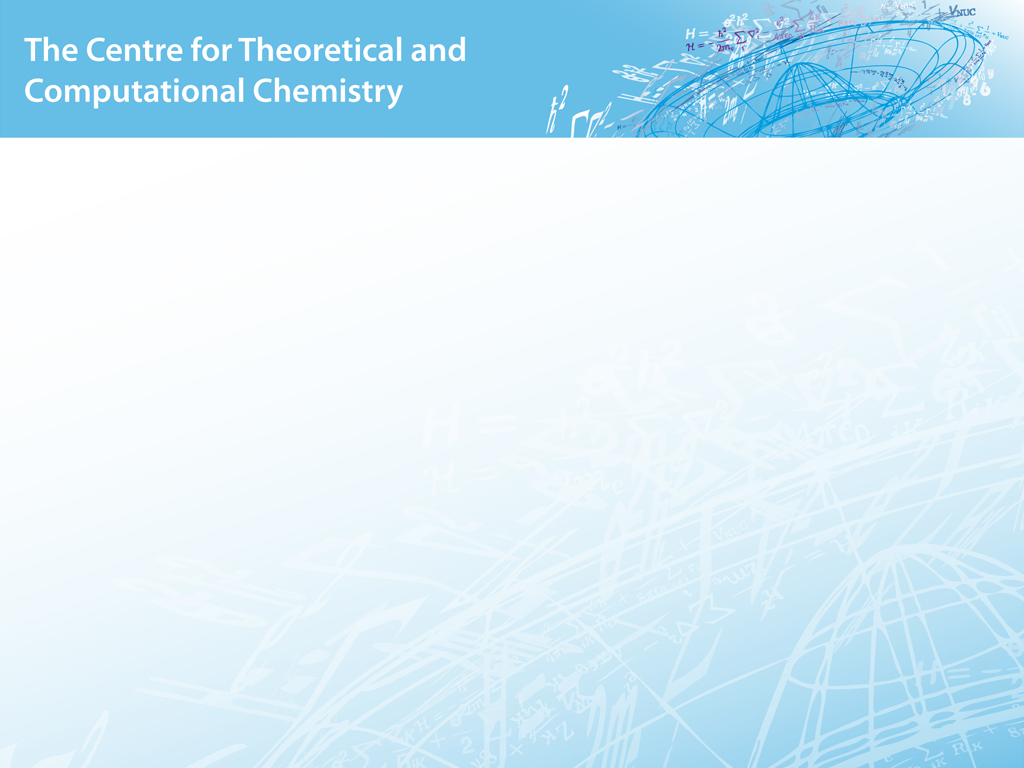
\includegraphics[width=1.02\paperwidth] {figures/ctcc_forside.jpg}}
\maketitle
}


\begin{frame}
    \frametitle{Static linear response}
    \begin{columns}
    \begin{column}[b]{0.5\linewidth}
    \centering
    \textbf{Static perturbation}
    \begin{equation}
        \nonumber
        \hat{H} = \pert{\hamiltonian}{0} + \pert{\hamiltonian}{1}
    \end{equation}
    \end{column}

    \begin{column}[b]{0.5\linewidth}
    \centering
    \textbf{Perturbed orbitals}
    \begin{equation}
        \nonumber
        \orbital_i = \pert{\orbital_i}{0} + \pert{\orbital_i}{1}
    \end{equation}
    \end{column}
    \end{columns}

    \vspace{5mm}

    \centering
    \textbf{Perturbed Fock operator}
    \begin{align}
        \nonumber
        \pert{\fockOper}{1} &= \pert{\hamiltonian}{1} + \pert{\potential}{1}
    \end{align}

    \vspace{5mm}

    \centering
    \textbf{Sternheimer equations}
    \begin{equation}
        \nonumber
        \pert{\fockOper}{0}\ket{\pert{\orbital_i}{1}} +
        \pert{\fockOper}{1}\ket{\pert{\orbital_i}{0}} =
        \sum_j \pert{F_{ji}}{0}\ket{\pert{\orbital_j}{1}} + 
        \sum_j \pert{F_{ji}}{1}\ket{\pert{\orbital_j}{0}}
    \end{equation}

    \vspace{5mm}

    \centering
    \textbf{Integral form} $\lambda_{i} \approx \pert{F}{0}_{ii}$
    \begin{equation}
        \nonumber
        \ket{\pert{\orbital_i}{1}} = -2\hat{G}_i\bigg[
        \pert{\potential}{0}\ket{\pert{\orbital_i}{1}} -
        \sum_j \Big(\pert{F}{0}_{ji} - \Lambda_{ji}\Big)
        \ket{\pert{\orbital_j}{1}} +
        \Big(1 - \pert{\density}{0}\Big)
        \pert{\fockOper}{1}\ket{\pert{\orbital_i}{0}}
        \bigg]
    \end{equation}
\end{frame}

\begin{frame}
    \frametitle{Unperturbed system}
    \begin{columns}
    \begin{column}[b]{0.5\linewidth}
    \centering
    \textbf{Kohn-Sham equations}
    \begin{equation}
        \nonumber
        \fockOper\ket{\orbital_i} = \sum_j F_{ji}\ket{\orbital_j}
    \end{equation}
    \end{column}
    \begin{column}[b]{0.5\linewidth}
    \centering
    \textbf{Potential operator} $0 \leq \alpha \leq 1$
    \begin{equation}
        \nonumber
        \potential = \nuclear + \coulomb - \alpha\exchange + \xc
    \end{equation}
    \end{column}
    \end{columns}

    \vspace{5mm}

    \begin{columns}
    \begin{column}[b]{0.5\linewidth}
    \centering
    \textbf{Fock matrix}
    \begin{equation}
        \nonumber
        F_{ij} = \bra{\orbital_i}\kinetic + \potential\ket{\orbital_j}
    \end{equation}

    \vspace{8mm}

    \textbf{One-particle density matrix}
    \begin{equation}
        \nonumber
        \rho(r,r') = \sum_i \orbital_i(r)\orbital_i^\dag(r')
    \end{equation}
    \end{column}
    \begin{column}[b]{0.5\linewidth}

    \centering
    \textbf{Two-electron operators}
    \begin{align}
        \nonumber
        \coulomb \ket{\orbital_p} &= \int\frac{\rho(r',r')\orbital_p(r)}{|r-r'|} \ud r'\\
        \nonumber
        \exchange \ket{\orbital_p} &= \int\frac{\rho(r,r')\orbital_p(r')}{|r-r'|} \ud r'\\
        \nonumber
        \xc \ket{\orbital_p} &= \bigg[\frac{\delta E_{xc}}{\delta \rho}\big[\rho(r,r)\big]\bigg] \orbital_p(r) 
    \end{align}
    \end{column}
    \end{columns}

    \vspace{5mm}

    \centering
    \textbf{Integral form} $\lambda_{i} \approx F_{ii}$
    \begin{equation}
        \nonumber
        \ket{\orbital_i} = -2\hat{G}_i\bigg[\potential\ket{\orbital_i} -
        \sum_j \Big(F_{ji} - \Lambda_{ji}\Big)\ket{\orbital_j}\bigg]
    \end{equation}
\end{frame}

\begin{frame}
    \frametitle{Two-electron operators}
    \begin{columns}
    \begin{column}[b]{0.4\linewidth}
    \centering
    \textbf{Unperturbed}
    \begin{align}
        \nonumber
        \pert{\potential}{0} &= \pert{\coulomb}{0} -\alpha\pert{\exchange}{0} + \pert{\xc}{0}\\
        \nonumber & \\
        \nonumber
        \pert{\coulomb}{0} \ket{\orbital_p} &= \int\frac{\pert{\rho}{0}(r',r')\orbital_p(r)}{|r-r'|} \ud r'\\
        \nonumber
        \pert{\exchange}{0} \ket{\orbital_p} &= \int\frac{\pert{\rho}{0}(r,r')\orbital_p(r')}{|r-r'|} \ud r'\\
        \nonumber
        \pert{\xc}{0} \ket{\orbital_p} &= \bigg[\frac{\delta E_{xc}}{\delta\rho}\big[\pert{\rho}{0}\big]\bigg] \orbital_p(r) 
    \end{align}
    \end{column}
    \begin{column}[b]{0.6\linewidth}
    \centering
    \textbf{Perturbed}
    \begin{align}
        \nonumber
        \pert{\potential}{1} &= \pert{\coulomb}{1} -\alpha\pert{\exchange}{1} + \pert{\xc}{1}\\
        \nonumber & \\
        \nonumber
        \pert{\coulomb}{1} \ket{\orbital_p} &= \int\frac{\pert{\rho}{1}(r',r')\orbital_p(r)}{|r-r'|} \ud r'\\
        \nonumber
        \pert{\exchange}{1} \ket{\orbital_p} &= \int\frac{\pert{\rho}{1}(r,r')\orbital_p(r')}{|r-r'|} \ud r'\\
        \nonumber
        \pert{\xc}{1} \ket{\orbital_p} &= \bigg[\frac{\delta^2 E_{xc}}{\delta
        \rho^2}\big[\pert{\rho}{0}\big]*\pert{\rho}{1}\bigg] \orbital_p(r) 
    \end{align}
    \end{column}
    \end{columns}

    \vspace{5mm}

\only<1>{

    \vspace{31mm}

}

\only<2>{
    \centering
    \textbf{Coulomb}
    \begin{equation}
        \nonumber
        \pert{\coulomb}{1} \ket{\orbital_p} = 
        \bigg[\int \frac{\pert{\rho}{1}(r',r')}{4\pi|r-r'|}\ud r'\bigg]\orbital_p(r)
    \end{equation}

    \vspace{16.7mm}

}

\only<3>{
    \centering
    \textbf{Hartree-Fock exchange}
    \begin{align}
        \nonumber
        \pert{\exchange}{1} \ket{\orbital_p}
        &= \sum_i 
        \pert{\orbital_i}{1}(r) \int
        \frac{\orbital_i^{(0)\dagger}(r')\orbital_p(r')}{4\pi|r-r'|} \ud r' \\
        \nonumber
        &+ \sum_i 
        \pert{\orbital_i}{0}(r) \int
        \frac{\orbital_i^{(1)\dagger}(r')\orbital_p(r')}{4\pi|r-r'|} \ud r'
    \end{align}

    \vspace{4.4mm}

}

\only<4>{
    \centering
    \textbf{Exchange-Correlation} $\gamma = \nabla\rho\cdot\nabla\rho$
    \begin{align}
        \nonumber
        \pert{\xc}{1} \ket{\orbital_p}
        = \bigg[&
        \frac{\partial^2 F_{xc}}{\partial \rho^2}\pert{\rho}{1} +
        2\frac{\partial^2 F_{xc}}{\partial \rho \partial \gamma}
        \Big(\nabla\pert{\rho}{0}\cdot\nabla\pert{\rho}{1}\Big) -\\
        \nonumber
        &\nabla\cdot\bigg(
        \Big(\nabla\pert{\rho}{0}\Big)
        \Big[
        2\frac{\partial^2 F_{xc}}{\partial\rho\partial\gamma}\pert{\rho}{1} +
        4\frac{\partial^2 F_{xc}}{\partial\gamma^2}
        \Big(\nabla\pert{\rho}{0}\cdot\nabla\pert{\rho}{1}\Big)
        \Big]
        \bigg) -\\
        \nonumber
        &\nabla\cdot\bigg(
        \Big(\nabla\pert{\rho}{1}\Big)\frac{\partial F_{xc}}{\partial\gamma}
        \bigg)
        \bigg] \ket{\orbital_p}
    \end{align}
}
\end{frame}

\begin{frame}
\frametitle{Magnetic linear response}
\centering
\textbf{Sternheimer equations}
\begin{equation}
    \nonumber
    \ket{\pert{\orbital_i}{1}} = -2\hat{G}_i\bigg[
    \pert{\potential}{0}\ket{\pert{\orbital_i}{1}} -
    \sum_j \Big(\pert{F}{0}_{ji} - \pert{\Lambda}{0}_{ji}\Big)
    \ket{\pert{\orbital_j}{1}} +
    \Big(1 - \pert{\density}{0}\Big)
    \pert{\fockOper}{1}\ket{\pert{\orbital_i}{0}}
    \bigg]
\end{equation}

\vspace{5mm}

\only<1>{
\textbf{Perturbed Fock operator}
\begin{equation}
    \nonumber
    \hat{F}^{(B)} = \hat{h}^{(B)} + \hat{J}^{(1)} - \alpha\hat{K}^{(1)} +
    \hat{V}_{xc}^{(1)}
\end{equation}
}

\only<2>{
\textbf{Perturbed Fock operator}
\begin{equation}
    \nonumber
    \hat{F}^{(B)} = \hat{h}^{(B)} + \cancel{\hat{J}^{(1)}} - \alpha\hat{K}^{(1)} +
    \cancel{\hat{V}_{xc}^{(1)}}
\end{equation}
}

\vspace{5mm}

\textbf{Perturbed density vanishes for imaginary (static) perturbations}
\begin{equation}
    \nonumber
    \pert{\rho}{B}(r,r) = \sum_i 
    \bigg[
    \orbital_i^{(0)}(r)\orbital_i^{(B)\dagger}(r) +
    \orbital_i^{(B)}(r)\orbital_i^{(0)\dagger}(r)
    \bigg]
    \equiv 0
\end{equation}

\vspace{5mm}

\pause
\begin{columns}
\begin{column}[b]{0.1\linewidth}
\end{column}
\begin{column}[b]{0.9\linewidth}
\begin{itemize}
    \item   Pure functionals ($\alpha=0$): \textbf{no two-electron contributions}
    \item   Fundamental defect of standard DFT: \textbf{no current dependence}
\end{itemize}
\end{column}
\end{columns}
\end{frame}


\begin{frame}
\frametitle{Magnetic properties}

\centering
\textbf{Second order property}
\begin{equation}
    \nonumber
    M = \left. \frac{\ud^2 E}{\ud b \ud a}\right|_{a,b=0}
\end{equation}

\vspace{8mm}

\begin{columns}
\begin{column}[b]{0.2\linewidth}
\end{column}

\begin{column}[b]{0.6\linewidth}
\begin{itemize}
    \item External magnetic field $\boldsymbol{B}$
    \item Nuclear magnetic moment $\boldsymbol{M}_K$ of nucleus $K$
\end{itemize}
\end{column}

\begin{column}[b]{0.2\linewidth}
\end{column}
\end{columns}

\vspace{13mm}

\begin{columns}
\begin{column}[b]{0.3\linewidth}
    \centering
    \textbf{Magnetizability tensor}
    \begin{equation}
        \nonumber
        \xi = \left. \frac{\ud^2 E}{\ud \boldsymbol{B} \ud \boldsymbol{B}}\right|_{\boldsymbol{B}=0}
    \end{equation}
\end{column}

\begin{column}[b]{0.4\linewidth}
    \centering
    \textbf{NMR shielding tensor}
    \begin{equation}
        \nonumber
        \sigma_K = \left. \frac{\ud^2 E}{\ud \boldsymbol{M}_K \ud
        \boldsymbol{B}}\right|_{\boldsymbol{M}_K,\boldsymbol{B}=0}
    \end{equation}
\end{column}

\begin{column}[b]{0.4\linewidth}
    \centering
    \textbf{Spin-spin coupling tensor}
    \begin{equation}
        \nonumber
        K_{KL} = \left. \frac{\ud^2 E}{\ud \boldsymbol{M}_K\ud
        \boldsymbol{M}_L}\right|_{\boldsymbol{M}_K,\boldsymbol{M}_L=0}
    \end{equation}
\end{column}
\end{columns}

\end{frame}


\begin{frame}
\frametitle{Magnetic properties}

\begin{columns}
\begin{column}[b]{0.48\linewidth}
    \centering
    \textbf{First-order interaction}
    \begin{equation}
        \nonumber
        \hat{h}^{(a)} = 
        \left. \frac{\ud \hat{H}}{\ud a}\right|_{a=0}
    \end{equation}
\end{column}

\begin{column}[b]{0.48\linewidth}
    \centering
    \textbf{Second-order interaction}
    \begin{equation}
        \nonumber
        \hat{h}^{(a,b)} = 
        \left. \frac{\ud^2 \hat{H}}{\ud b \ud a}\right|_{a,b=0}
    \end{equation}
\end{column}
\end{columns}

\vspace{5mm}

\centering
\textbf{First-order (paramagnetic) operators}
\begin{equation}
    \nonumber
    \hat{h}^{(B)} = \frac{1}{2}\sum_j^{el} \hat{l}_{jO} \qquad \qquad \qquad
    \hat{h}^{(M_K)} = \alpha^2 \sum_j^{el} \frac{\hat{l}_{jK}}{r_{jK}^3}
\end{equation}

\vspace{5mm}

\textbf{Second-order (diamagnetic) operators}
\begin{align}
    \nonumber
    \hat{h}^{(B,B)} &= 
    \sum_j^{el} \left(r_{jO}\cdot r_{jO}\right)1 - r_{jO}r_{jO}^T\\
    \nonumber
    \hat{h}^{(B,M_K)} &= \frac{\alpha^2}{2} 
    \sum_j^{el} \frac{\left(r_{jO}\cdot r_{jK}\right)1 -
    r_{jO}r_{jK}^T}{r_{jK}^3}
\end{align}

\end{frame}

\begin{frame}
\frametitle{Magnetic properties}
\centering
\textbf{Traditional formulation}
\begin{equation}
    \nonumber
    M = \bra{0}\pert{\hamiltonian}{a,b}\ket{0} - 2\sum_{n \neq 0}
    \frac{\bra{0}\pert{\hamiltonian}{a}\ket{n}\bra{n}\pert{\hamiltonian}{b}\ket{0}}
    {E_n - E_0}
\end{equation}

\vspace{7mm}

\textbf{Density matrix formulation}
\begin{equation}
    \nonumber
    M = Tr\Big[\pert{D}{0}\pert{h}{a,b}\Big] + Tr\Big[\pert{D}{a}\pert{h}{b}\Big]
\end{equation}

\vspace{7mm}

\textbf{Real-space formulation}
\begin{equation}
    \nonumber
    M = 
    \int \pert{\density}{0}\pert{\hamiltonian}{a,b} \ud r +
    \int \pert{\density}{a}\pert{\hamiltonian}{b} \ud r
\end{equation}
\begin{equation}
    \nonumber
    M = \sum_i
    \bra{\pert{\orbital_i}{0}}\pert{\hamiltonian}{a,b}\ket{\pert{\orbital_i}{0}} 
    + \sum_i \bigg[
    \bra{\pert{\orbital_i}{0}}\pert{\hamiltonian}{b}\ket{\pert{\orbital_i}{a}} +
    \bra{\pert{\orbital_i}{a}}\pert{\hamiltonian}{b}\ket{\pert{\orbital_i}{0}}
    \bigg]
\end{equation}

\end{frame}

\begin{frame}
\frametitle{Magnetic properties}
\centering
\textbf{Magnetizability tensor}
\begin{align}
    \nonumber
    \xi_{\mu\nu}
    &= \int \pert{\density}{0}\pert{\hamiltonian}{B,B}_{\mu\nu} \ud r
    +  \int \pert{\density}{B}_{\mu}\pert{\hamiltonian}{B}_{\nu} \ud r
\end{align}

\vspace{5mm}

\textbf{NMR shielding tensor}
\begin{align}
    \nonumber
    \big[\sigma_K\big]_{\mu\nu}
    &= \int \pert{\density}{0}\pert{\hamiltonian}{B,M_K}_{\mu\nu} \ud r
    +  \int \pert{\density}{B}_{\mu}\pert{\hamiltonian}{M_K}_{\nu} \ud r
\end{align}

\vspace{5mm}

\begin{itemize}
    \item   $\mu,\nu=x,y,z$ are components of the perturbing fields
    \item   $\xi$ and $\sigma_K$ of \textbf{all} nuclei computed from the
            \textbf{same} perturbed density $\pert{\density}{B}$
    \item   $\pert{\density}{B}_\mu$ means density perturbed by
            $\pert{\hamiltonian}{B}_\mu$, e.i. the magnetic field component $B_\mu$
    \item   For NMR shieldings, the order of the perturbations can be swapped
\end{itemize}
\end{frame}

\begin{frame}
\frametitle{Magnetic linear response}
\centering
\textbf{Sternheimer equations}
\begin{equation}
    \nonumber
    \ket{\pert{\orbital_i}{1}} = -2\hat{G}_i\bigg[
    \pert{\potential}{0}\ket{\pert{\orbital_i}{1}} -
    \sum_j \Big(\pert{F}{0}_{ji} - \pert{\Lambda}{0}_{ji}\Big)
    \ket{\pert{\orbital_j}{1}} +
    \Big(1 - \pert{\density}{0}\Big)
    \pert{\fockOper}{1}\ket{\pert{\orbital_i}{0}}
    \bigg]
\end{equation}

\vspace{5mm}

\only<1>{
\textbf{Perturbed Fock operator}
\begin{equation}
    \nonumber
    \hat{F}^{(B)} = \hat{h}^{(B)} + \hat{J}^{(1)} - \alpha\hat{K}^{(1)} +
    \hat{V}_{xc}^{(1)}
\end{equation}
}

\only<2>{
\textbf{Perturbed Fock operator}
\begin{equation}
    \nonumber
    \hat{F}^{(B)} = \hat{h}^{(B)} + \cancel{\hat{J}^{(1)}} - \alpha\hat{K}^{(1)} +
    \cancel{\hat{V}_{xc}^{(1)}}
\end{equation}
}

\vspace{5mm}

\textbf{Perturbed density vanishes for imaginary (static) perturbations}
\begin{equation}
    \nonumber
    \pert{\rho}{B}(r,r) = \sum_i 
    \bigg[
    \orbital_i^{(0)}(r)\orbital_i^{(B)\dagger}(r) +
    \orbital_i^{(B)}(r)\orbital_i^{(0)\dagger}(r)
    \bigg]
    \equiv 0
\end{equation}

\vspace{5mm}

\pause
\begin{itemize}
    \item   Pure functionals ($\alpha=0$): \textbf{no two-electron contributions}
    \item   Fundamental defect of standard DFT: \textbf{no current dependence}
\end{itemize}

\end{frame}


\begin{frame}
    \frametitle{Results}
    Accuracy
    Origin dependence
\end{frame}

\begin{frame}
\frametitle{Magnesium Oxide}
   
\centering
\textbf{Hartree-Fock shielding constant (ppm)}
\begin{table}
\begin{tabular}{crrr}
\hline
\hline
    &              &            &             \\
    &              &
\multicolumn{1}{c}{$\sigma(Mg)$}              &
\multicolumn{1}{c}{$\sigma(O)$}	              \\
    &              &            &             \\
MW  & $10^{-4}$    &  1538.9211 & -16726.3490 \\
    & $10^{-5}$    &  1584.1109 & -17466.4867 \\
    & $10^{-6}$    &  1578.7322 & -17358.6849 \\
    & $10^{-7}$    &  1579.4610 & -17375.4221 \\
    &              &            &             \\
GTO & pcS-4        &  1617.5056 & -18143.8405 \\
    & pcS-3        &  1757.7204 & -20822.5428 \\
    & pcS-2        &-19388.2423 & 386900.5044 \\
    & pcS-1        &    94.4529 &  11293.4315 \\
    & pcS-0        &   448.6993 &   4880.3077 \\
    &              &            &             \\
\hline
\hline
\end{tabular}
\end{table}

Frank Jensen's polarization consistent basis sets\\
GTO calculations with Dalton

\end{frame}

\begin{frame}
\frametitle{Benchmarking DFT functionals}
\centering
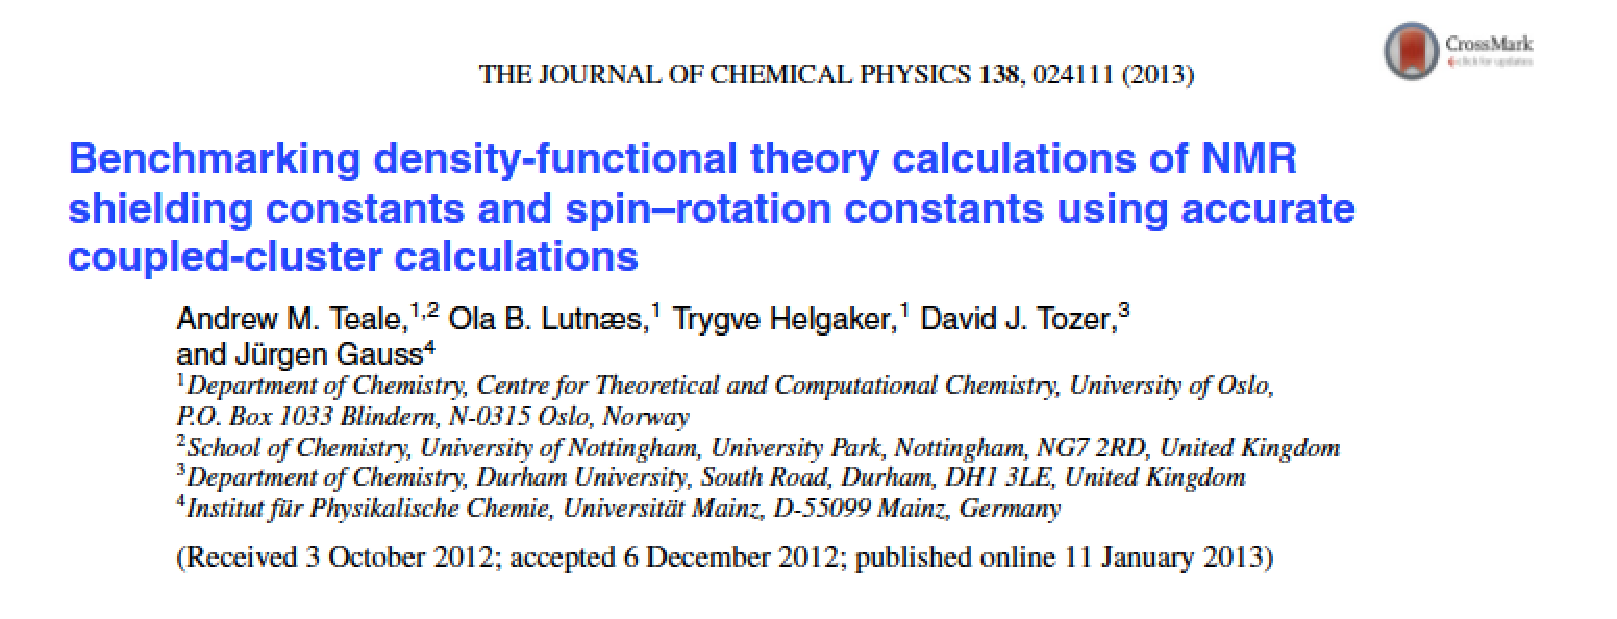
\includegraphics[scale=0.35]{figures/Teale_etal_2013.pdf}

\vspace{10mm}

\begin{columns}
\begin{column}[b]{0.5\textwidth}
    \textbf{Wave function methods}
    \begin{itemize}
        \item   RHF, CCSD, CCSD(T)
        \item   aug-cc-pCVXZ, X=D,T,Q
        \item   Basis set extrapolation
        \item   Comparison with experiment
    \end{itemize}
\end{column}
\begin{column}[b]{0.5\textwidth}
    \textbf{Density functional methods}
    \begin{itemize}
        \item   LDA, GGA, hybrid-GGA, OEP
        \item   aug-cc-pCVXZ, X=D,T,Q
        \item   Comparison with CCSD(T)
        \item   Comparison with experiment
    \end{itemize}
\end{column}
\end{columns}
\end{frame}

\begin{frame}
\frametitle{Benchmarking DFT functionals}

\vspace{13mm}

\centering
\textbf{Hartree-Fock extrapolation formula}
\begin{equation}
    \nonumber
    P_\infty = 
    \frac{P_X \exp{(\alpha X)} - P_Y \exp{(\alpha Y)}}
    {\exp{(\alpha X)} - \exp{(\alpha Y)}}
\end{equation}

\vspace{19mm}

\begin{columns}
\begin{column}[b]{0.5\textwidth}
    \textbf{Wave function methods}
    \begin{itemize}
        \item   RHF, CCSD, CCSD(T)
        \item   aug-cc-pCVXZ, X=D,T,Q
        \item   Basis set extrapolation
        \item   Comparison with experiment
    \end{itemize}
\end{column}
\begin{column}[b]{0.5\textwidth}
    \textbf{Density functional methods}
    \begin{itemize}
        \item   LDA, GGA, hybrid-GGA, OEP
        \item   aug-cc-pCVXZ, X=D,T,Q
        \item   Comparison with CCSD(T)
        \item   Comparison with experiment
    \end{itemize}
\end{column}
\end{columns}
\end{frame}

\begin{frame}
\frametitle{Benchmarking DFT functionals}

\centering
\textbf{Functionals}
\begin{multicols}{3}
\begin{itemize}
    \item Hartree-Fock
    \item LDA
    \item BLYP
    \item B3LYP
    \item PBE
    \item PBE0
\end{itemize}
\end{multicols}

\vspace{5mm}

\textbf{Molecules}
\begin{multicols}{4}
\begin{itemize}
    \item HF
    \item CO
    \item N$_2$
    \item H$_2$O
    \item HCN
    \item HOF
    \item O$_3$
    \item NH$_3$      
    \item CH$_2$O     
    \item CH$_4$      
    \item C$_2$H$_4$  
    \item AlF         
    \item CH$_3$F     
    \item C$_3$H$_4$  
    \item FCCH        
    \item FCN         
    \item H$_2$S      
    \item HCP         
    \item HFCO        
    \item H$_2$C$_2$O 
    \item LiF         
    \item LiH        
    \item N$_2$O     
    \item OCS        
    \item OF$_2$     
    \item H$_4$C$_2$O
    \item PN         
    \item SO$_2$     
\end{itemize}
\end{multicols}
\end{frame}

\begin{frame}
\frametitle{Comparison with Complete Basis Set limit}
\textbf{MW calculations}
\begin{itemize}
    \item   MRChem
    \item   MWX: $\epsilon=10^{-X}, X=3,4,5,6$
\end{itemize}

\vspace{5mm}

\textbf{GTO calculations}
\begin{itemize}
    \item   Teale \etal
    \item   XZ: aug-cc-pCVXZ, X = T,Q
    \item   $[$TQ$\alpha]$: Extrapolated aug-cc-pCV$[$TQ$]$Z with exponential
            parameter $\alpha$
\end{itemize}

\vspace{5mm}

\textbf{Error analysis}
\begin{itemize}
    \item   NMR shielding constant (ppm)
    \item   Average over all 28 molecules
    \item   MW6 is taken as CSB reference
\end{itemize}
\end{frame}

\begin{frame}
\frametitle{Comparison with Complete Basis Set limit}
\centering
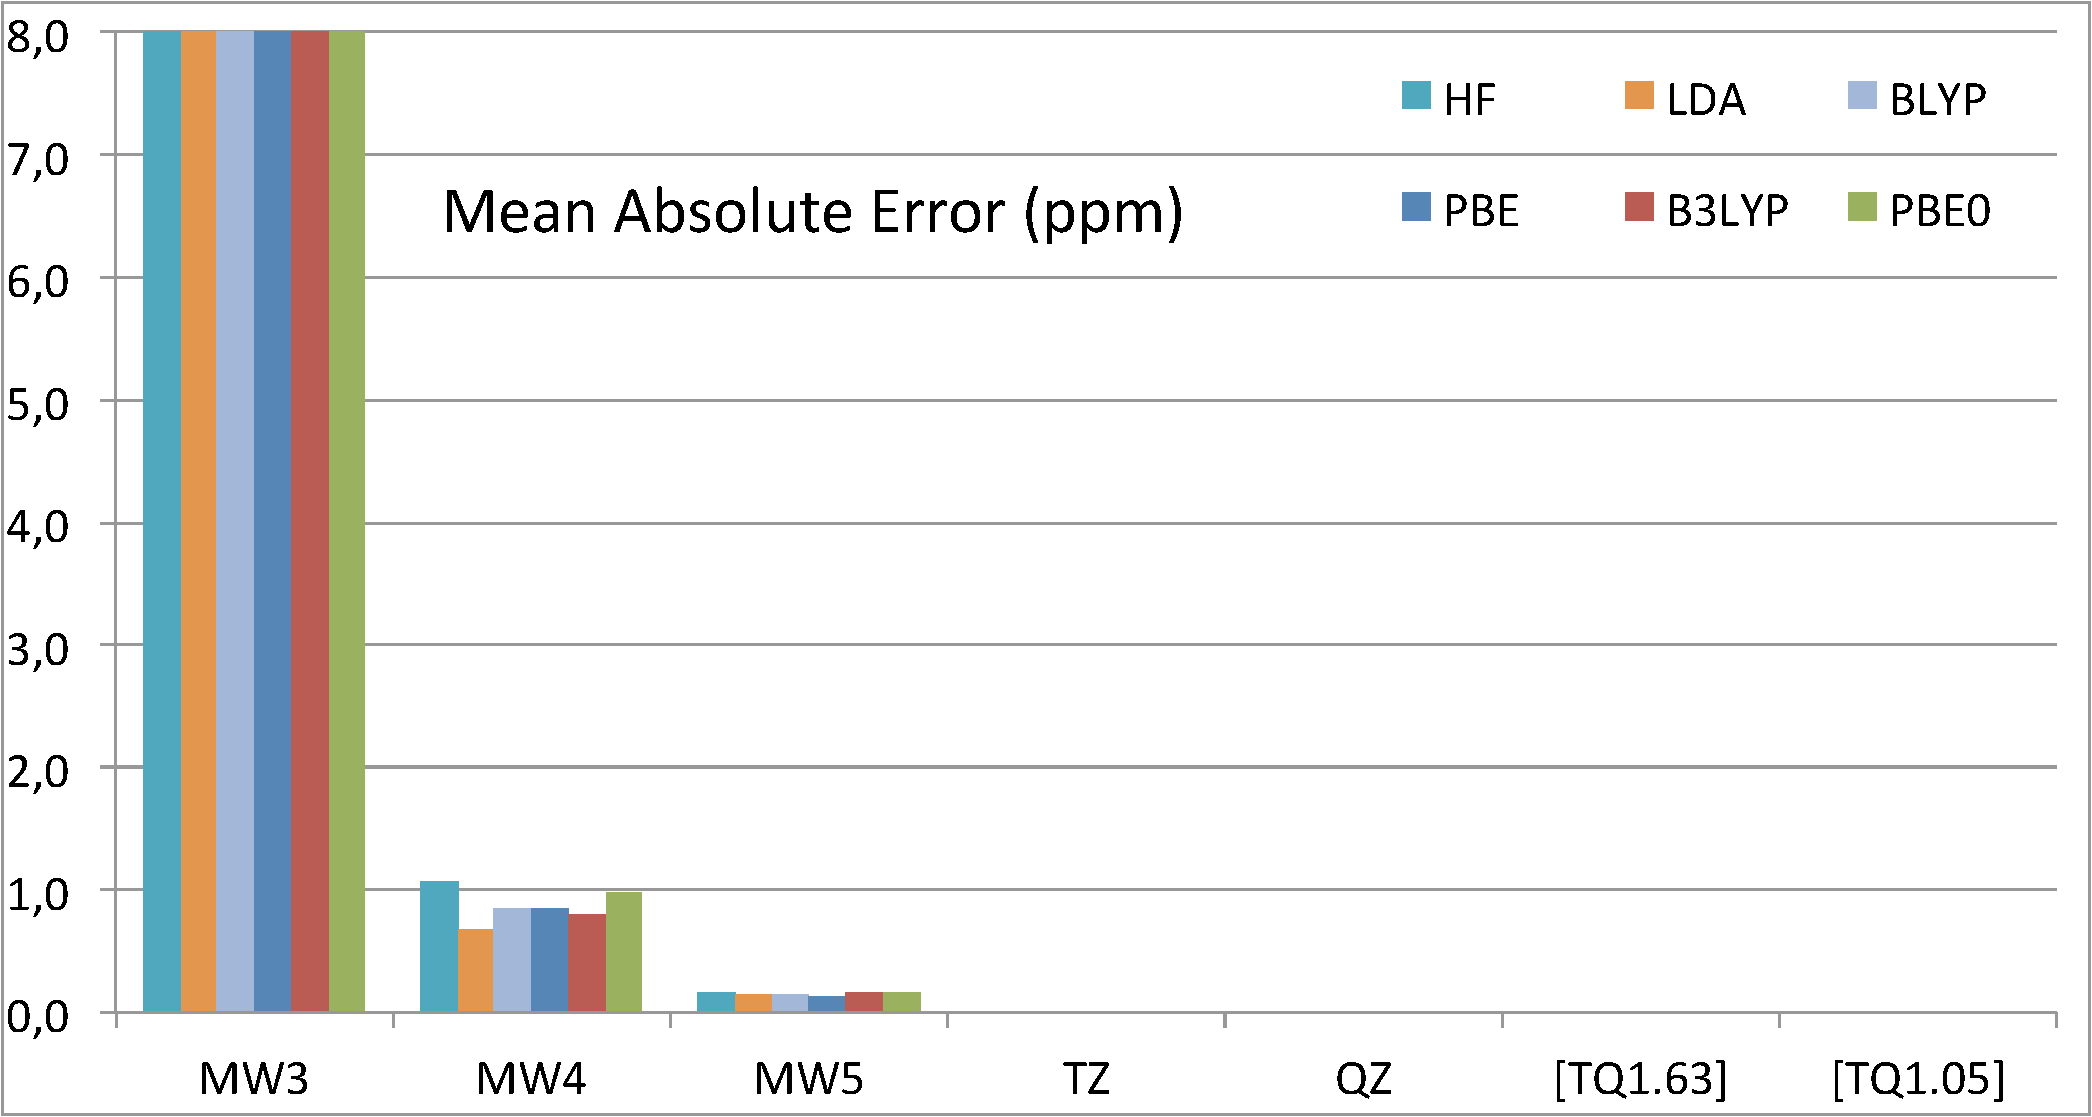
\includegraphics[scale=0.3]{figures/mae_bas_1.pdf}
\end{frame}

\begin{frame}
\frametitle{Comparison with Complete Basis Set limit}
\centering
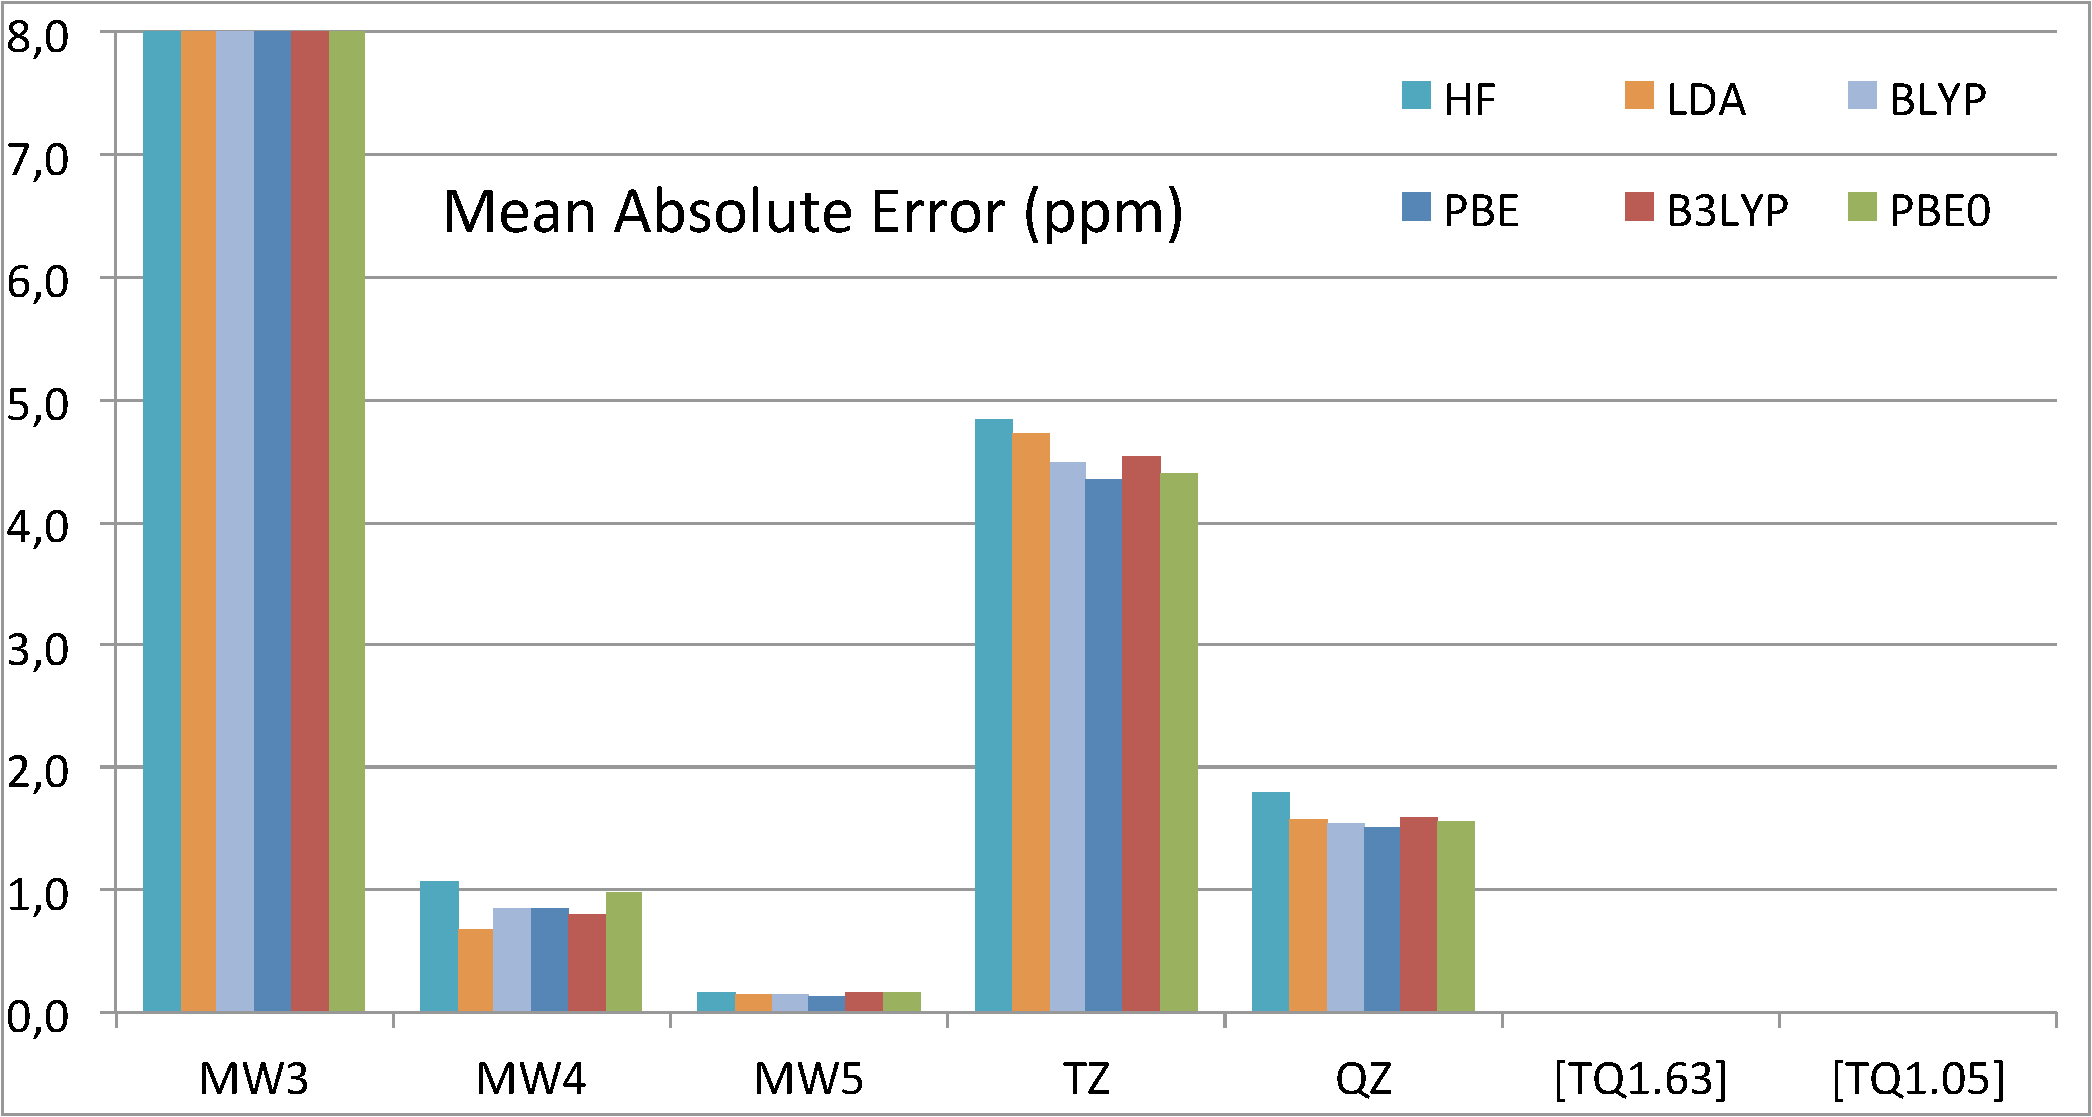
\includegraphics[scale=0.3]{figures/mae_bas_2.pdf}
\end{frame}

\begin{frame}
\frametitle{Comparison with Complete Basis Set limit}
\centering
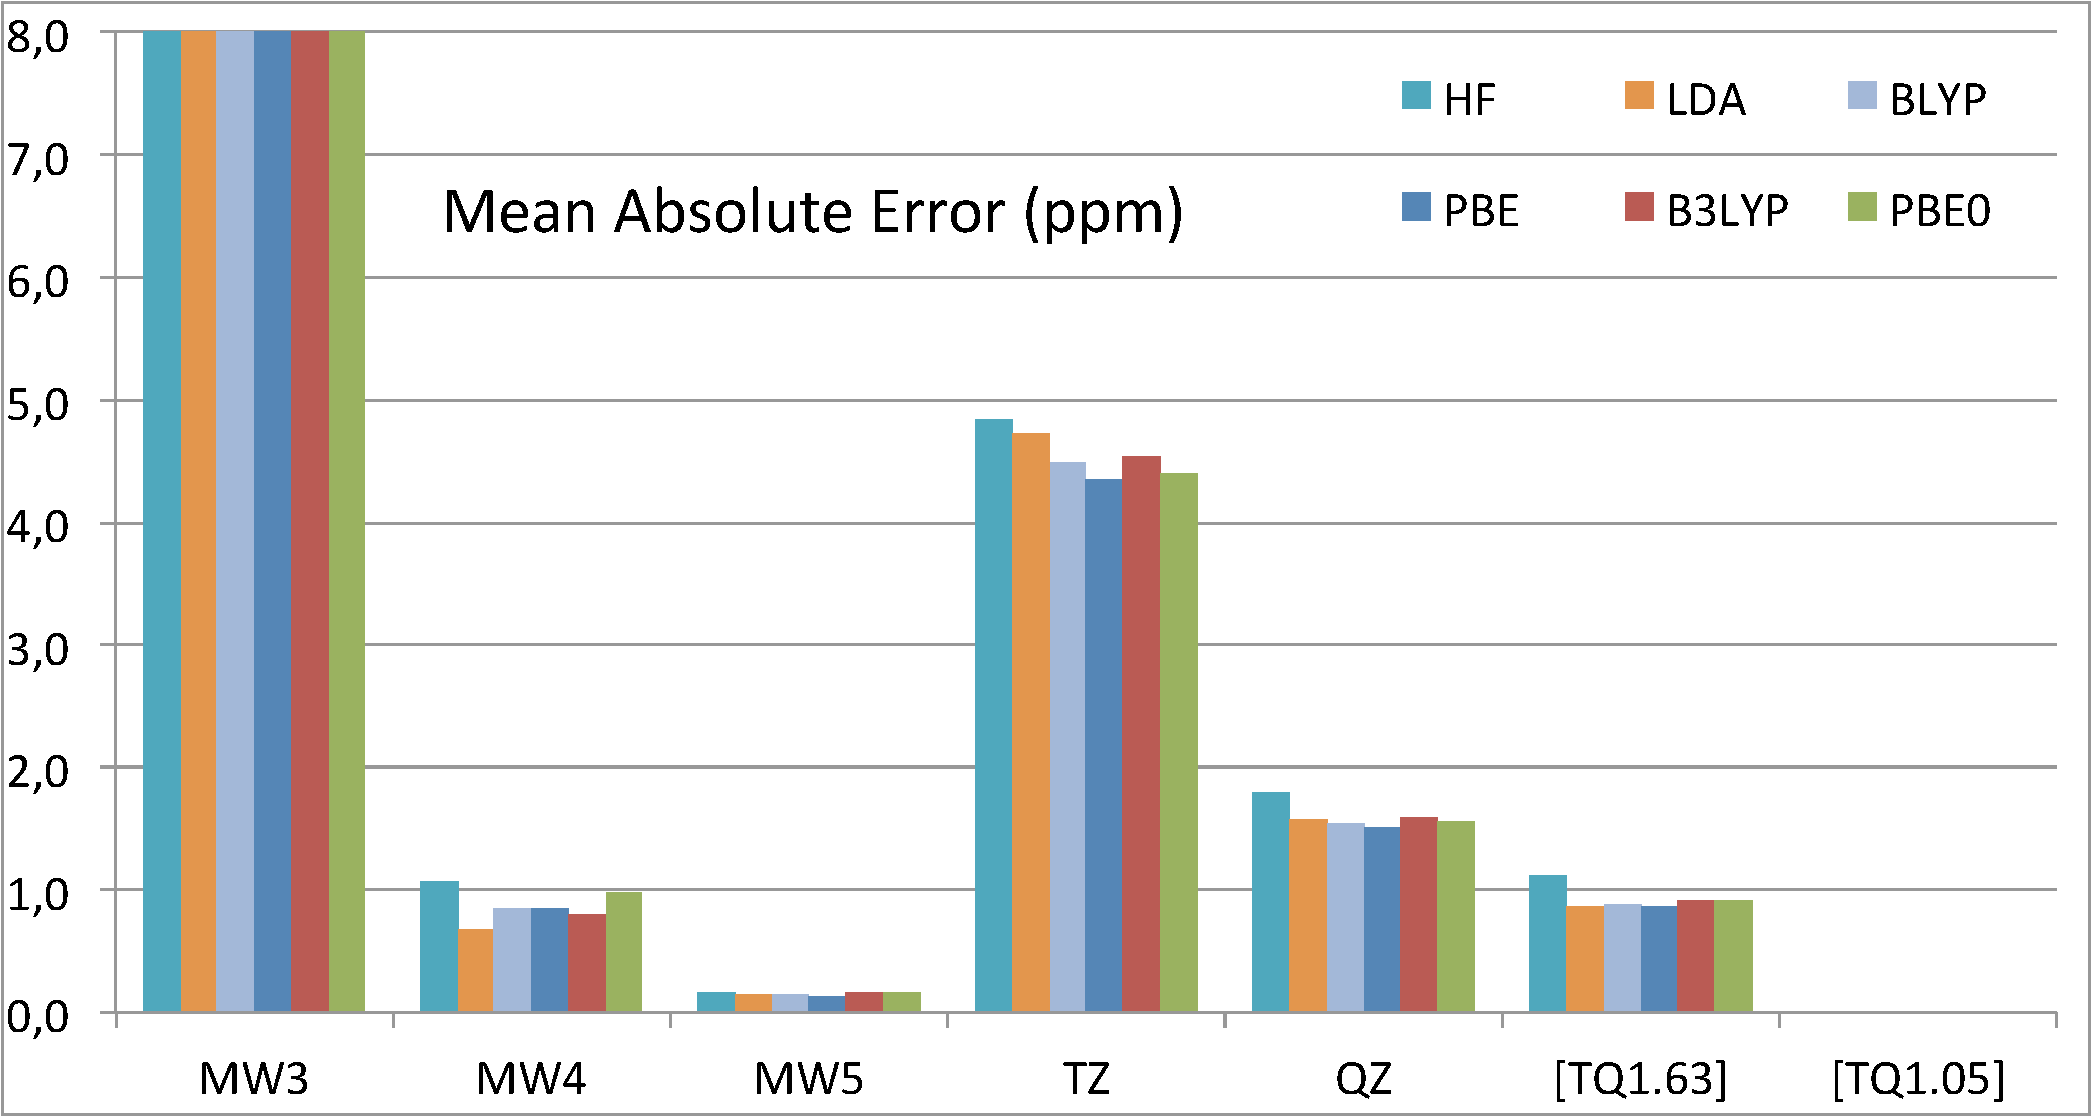
\includegraphics[scale=0.3]{figures/mae_bas_3.pdf}
\end{frame}

\begin{frame}
\frametitle{Comparison with Complete Basis Set limit}
\centering
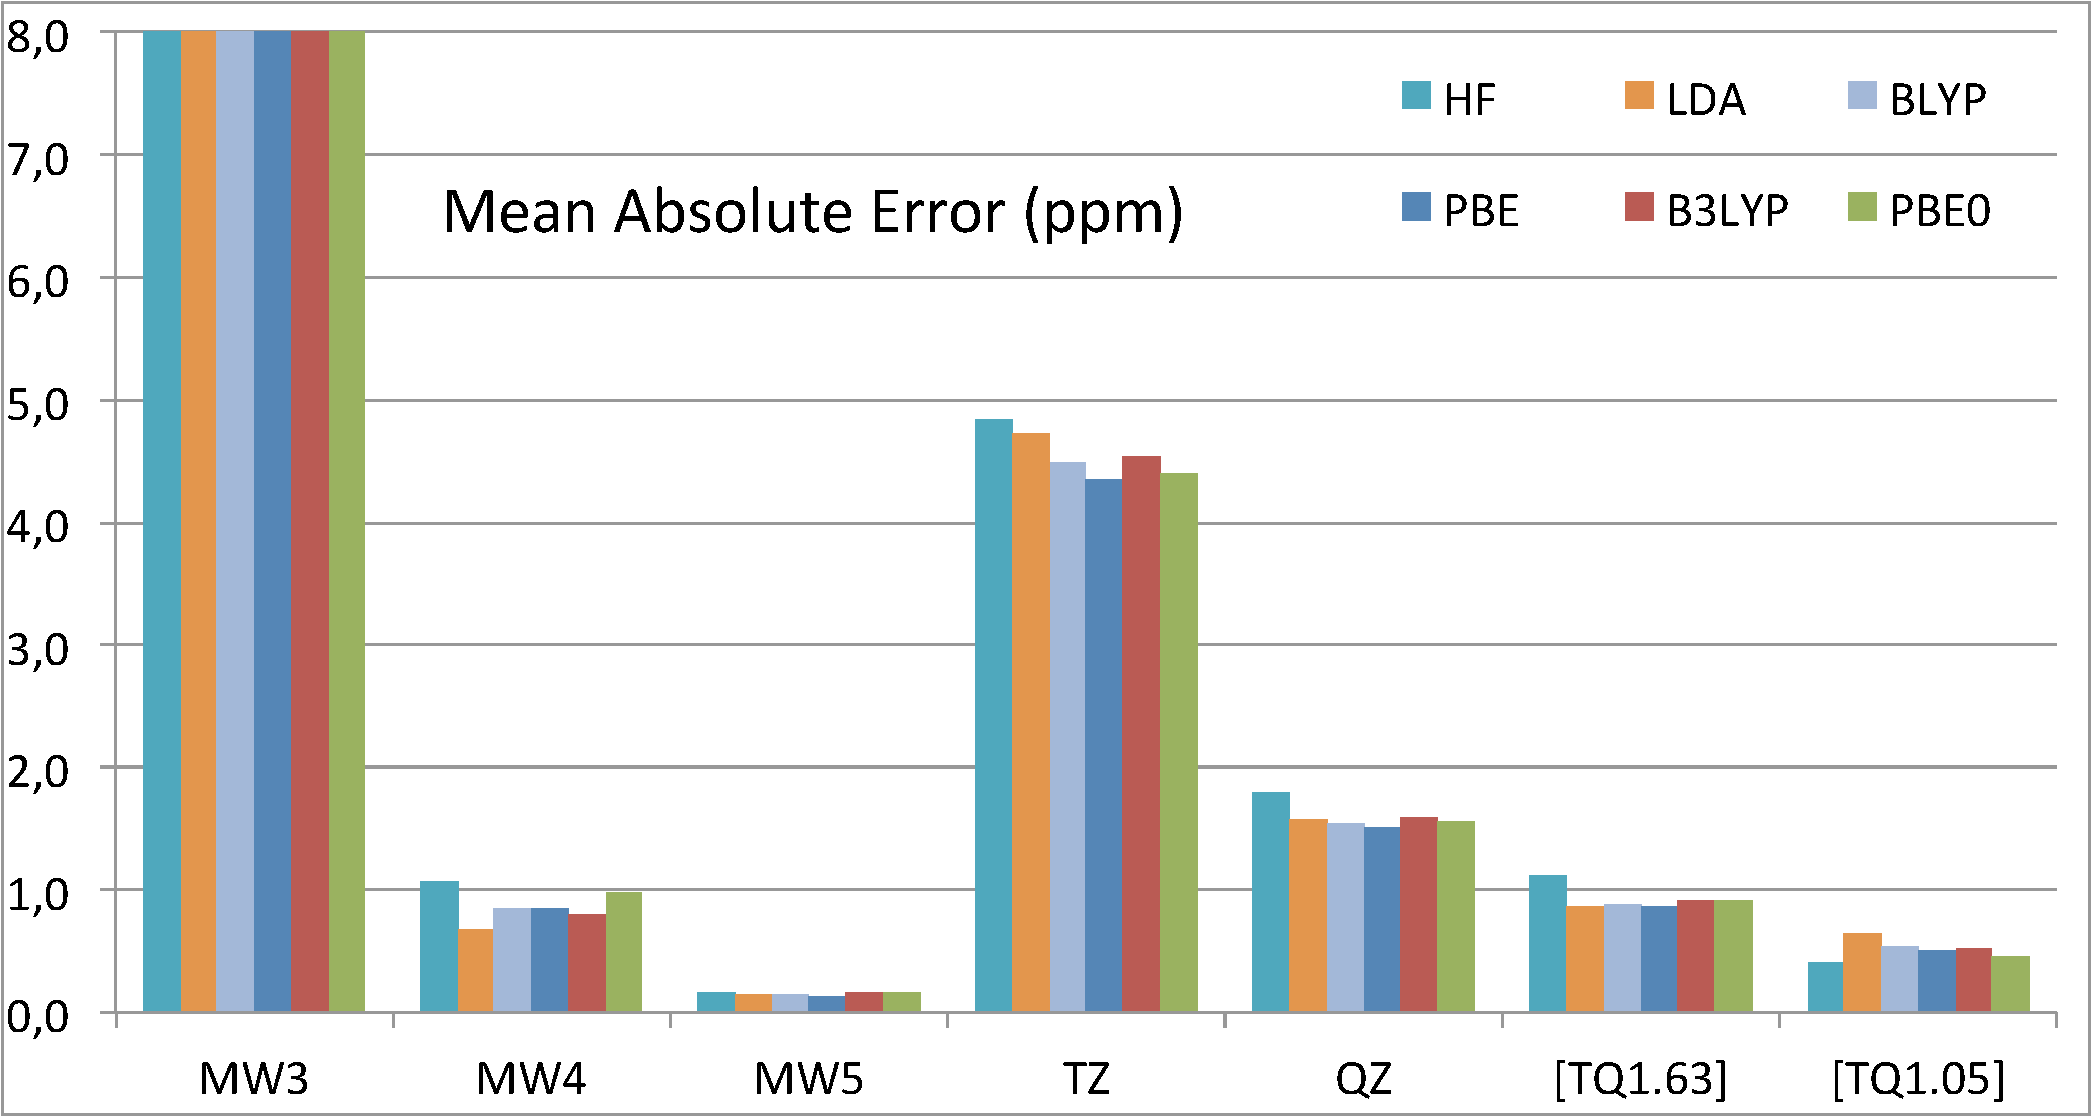
\includegraphics[scale=0.3]{figures/mae_bas_4.pdf}
\end{frame}

\begin{frame}
\frametitle{Computation time}
\textbf{MW calculations}
\begin{itemize}
    \item   MRChem
    \item   16/20 CPUs on Stallo
    \item   MWX: $\epsilon=10^{-X}, X=3,4,5,6$
\end{itemize}

\vspace{5mm}

\textbf{GTO calculations}
\begin{itemize}
    \item   Dalton
    \item   1 CPU on Stallo
    \item   XZ: aug-cc-pCVXZ, X = T,Q
\end{itemize}

\vspace{5mm}

\textbf{Timings}
\begin{itemize}
    \item   Average over all 28 molecules
    \item   4 SCF optimizations (ground-state + 3 response)
    \item   Minutes wall-time on 16 CPUs (renormalized)
\end{itemize}
\end{frame}

\begin{frame}
\frametitle{Computation time}
\centering
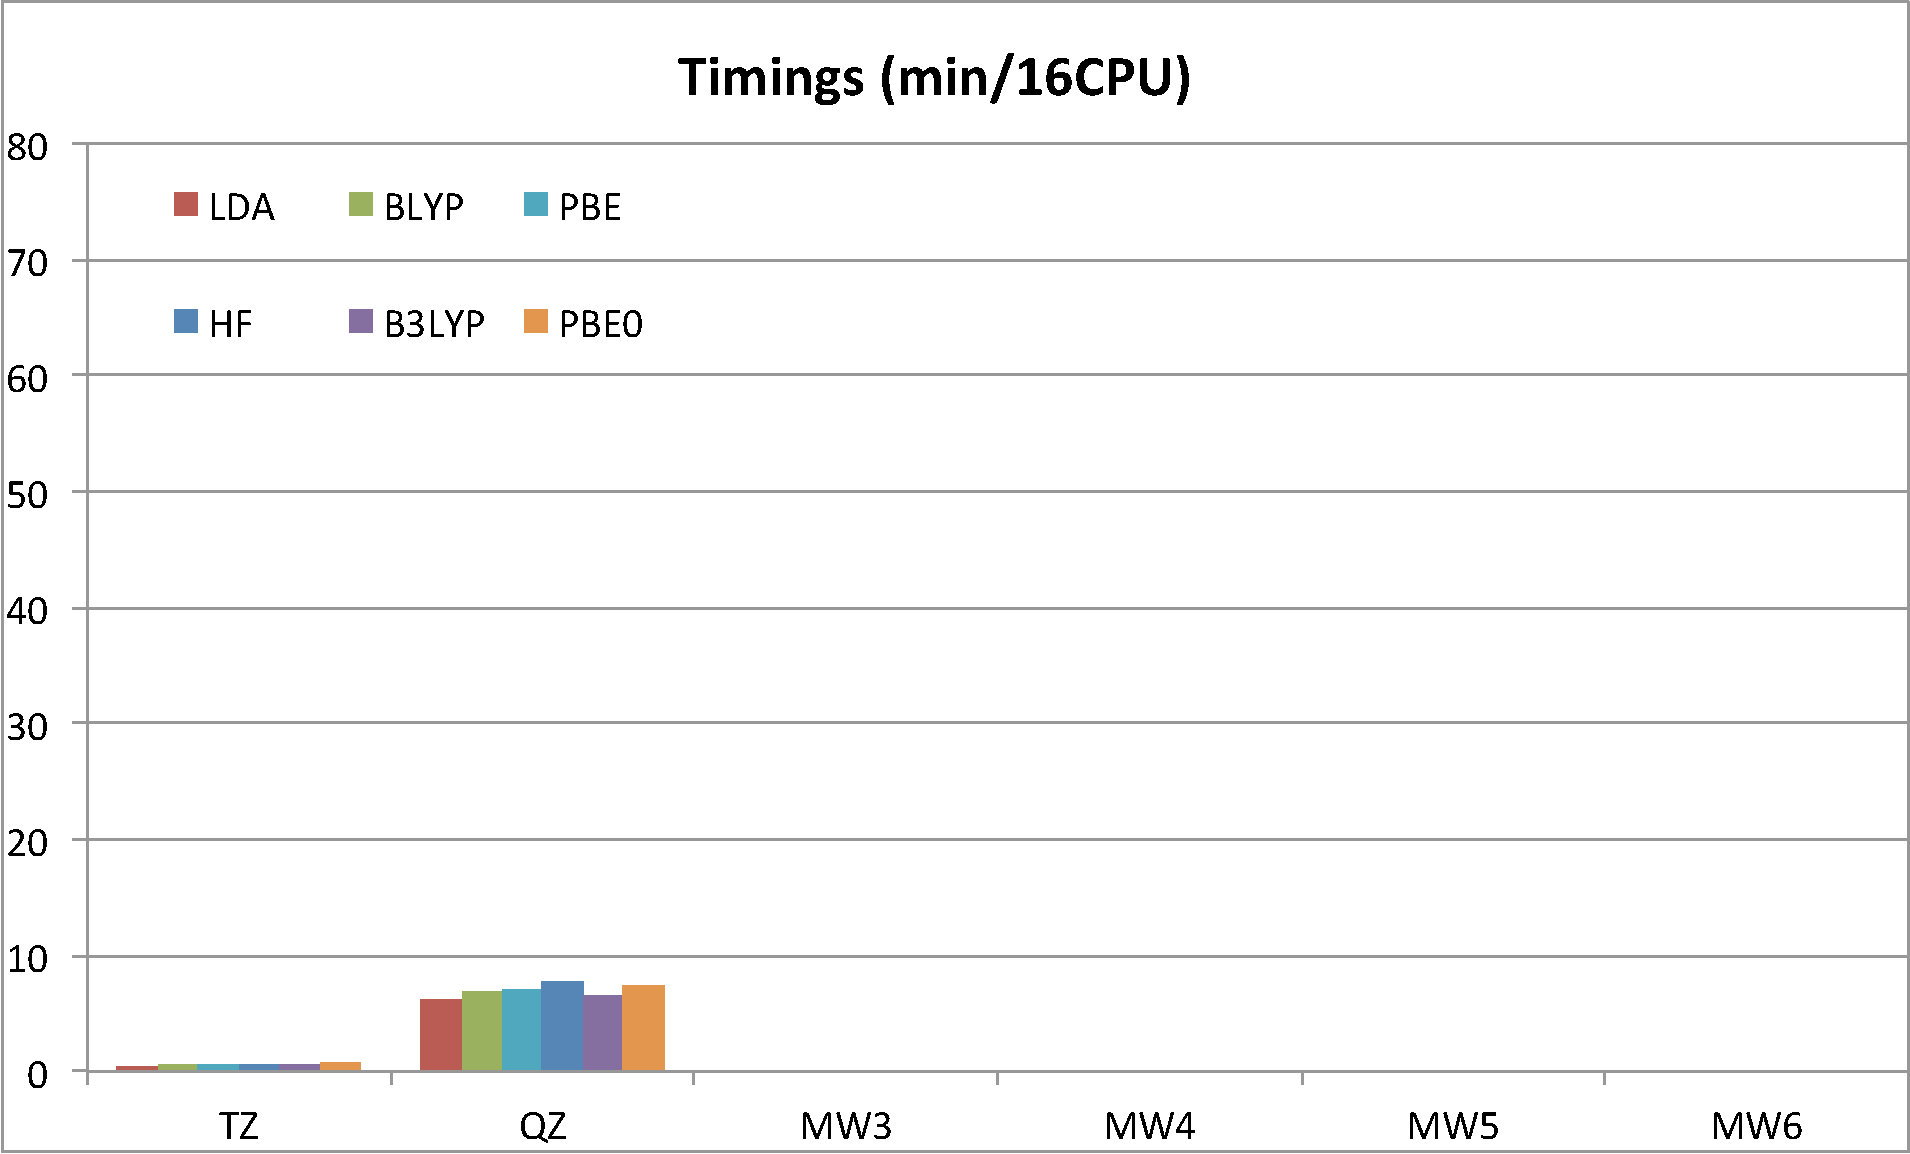
\includegraphics[scale=0.3]{figures/time_1.pdf}
\end{frame}

\begin{frame}
\frametitle{Computation time}
\centering
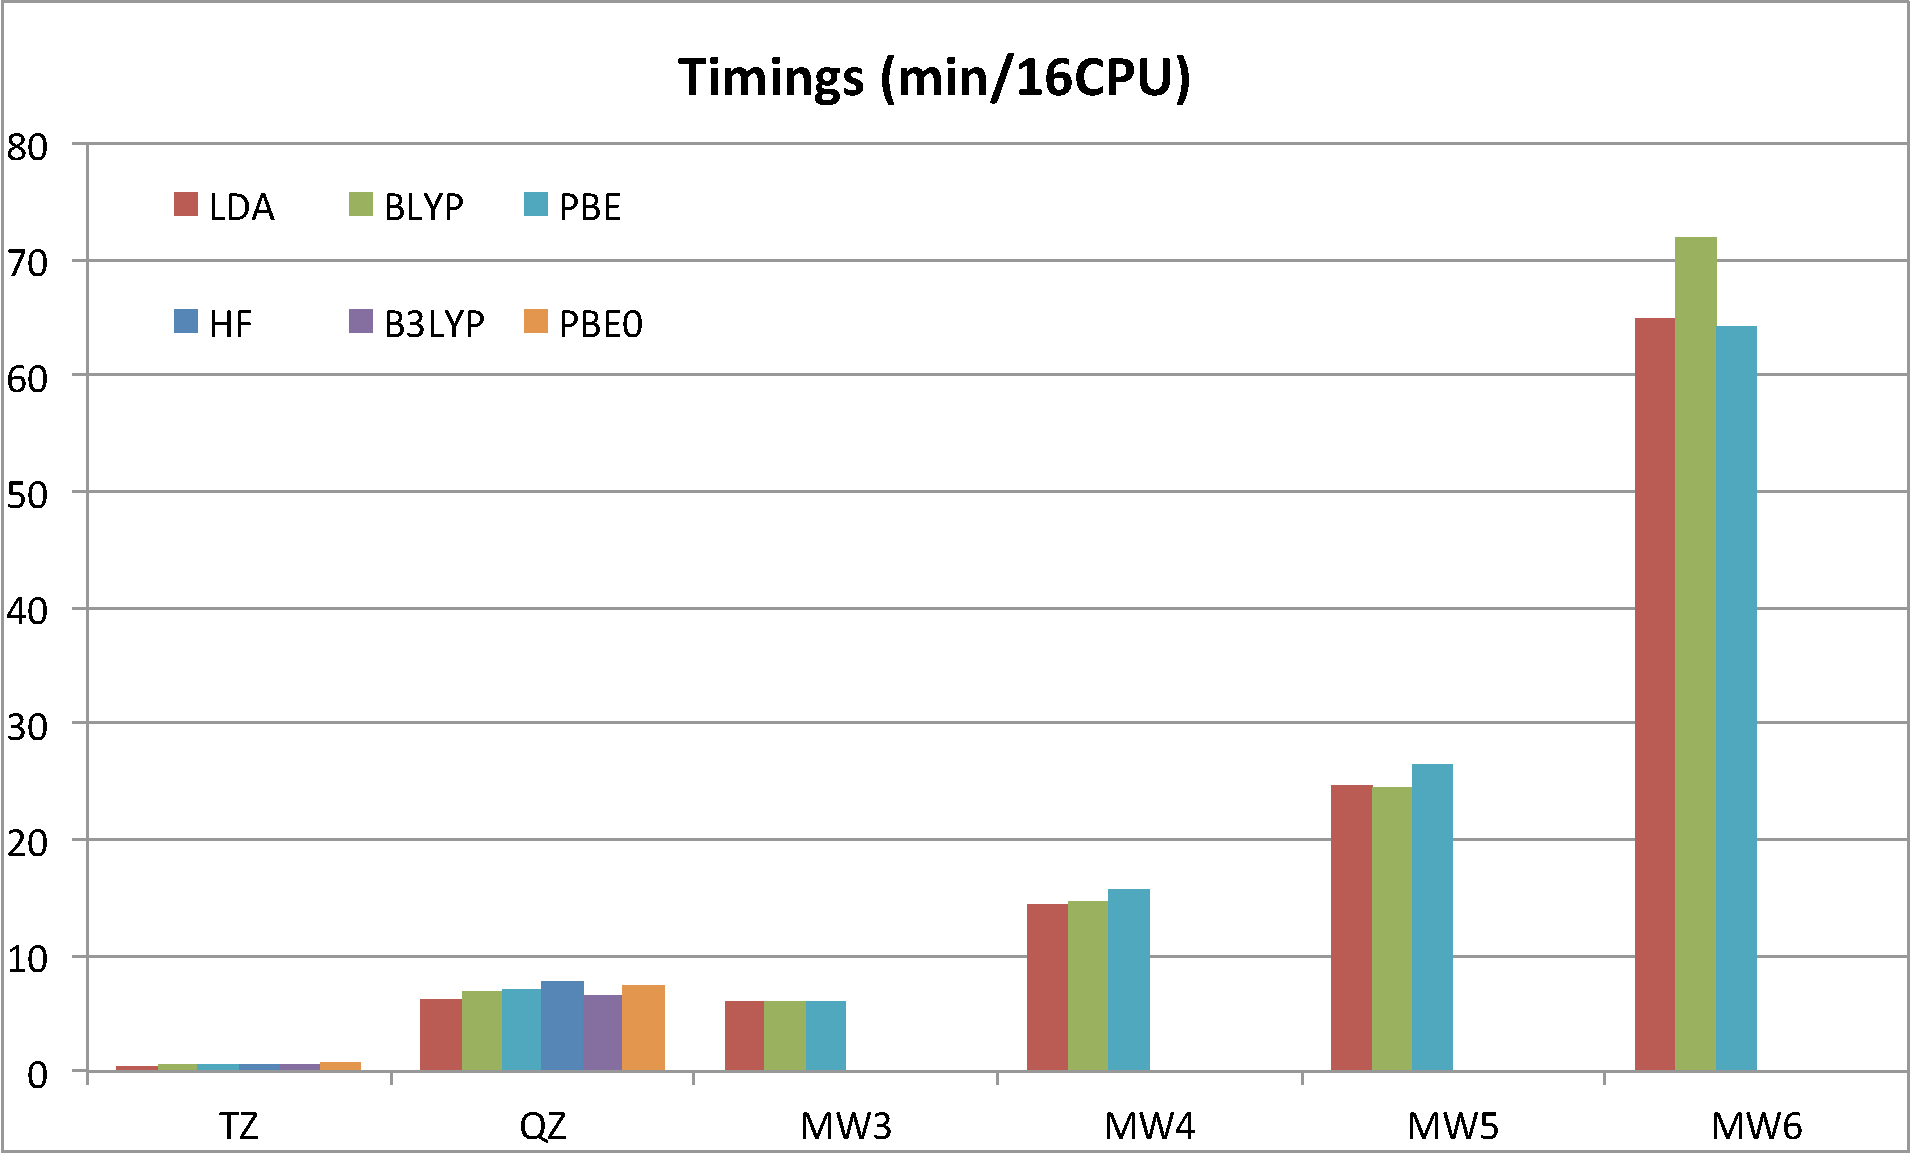
\includegraphics[scale=0.3]{figures/time_2.pdf}
\end{frame}

\begin{frame}
\frametitle{Computation time}
\centering
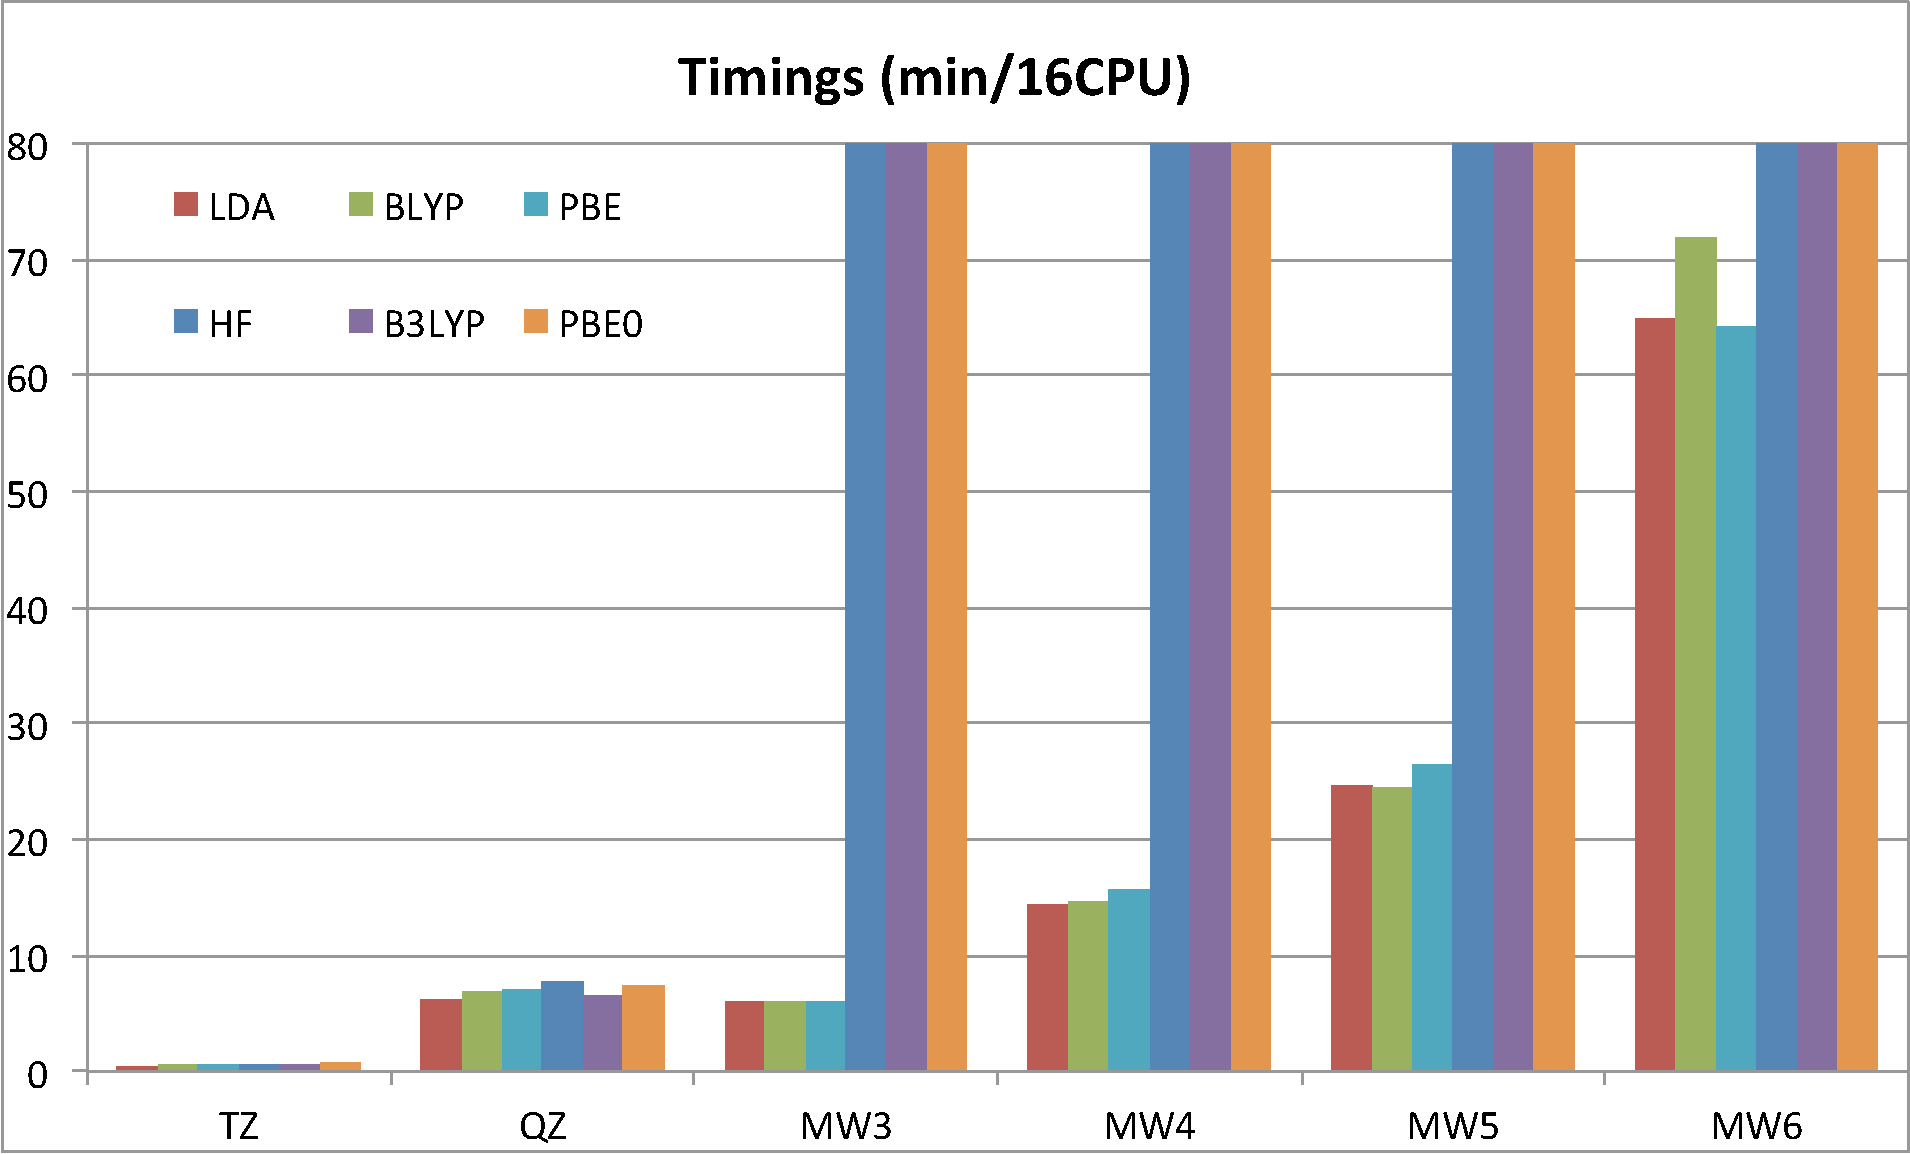
\includegraphics[scale=0.3]{figures/time_3.pdf}
\end{frame}

\begin{frame}
\frametitle{Computation time}
\centering
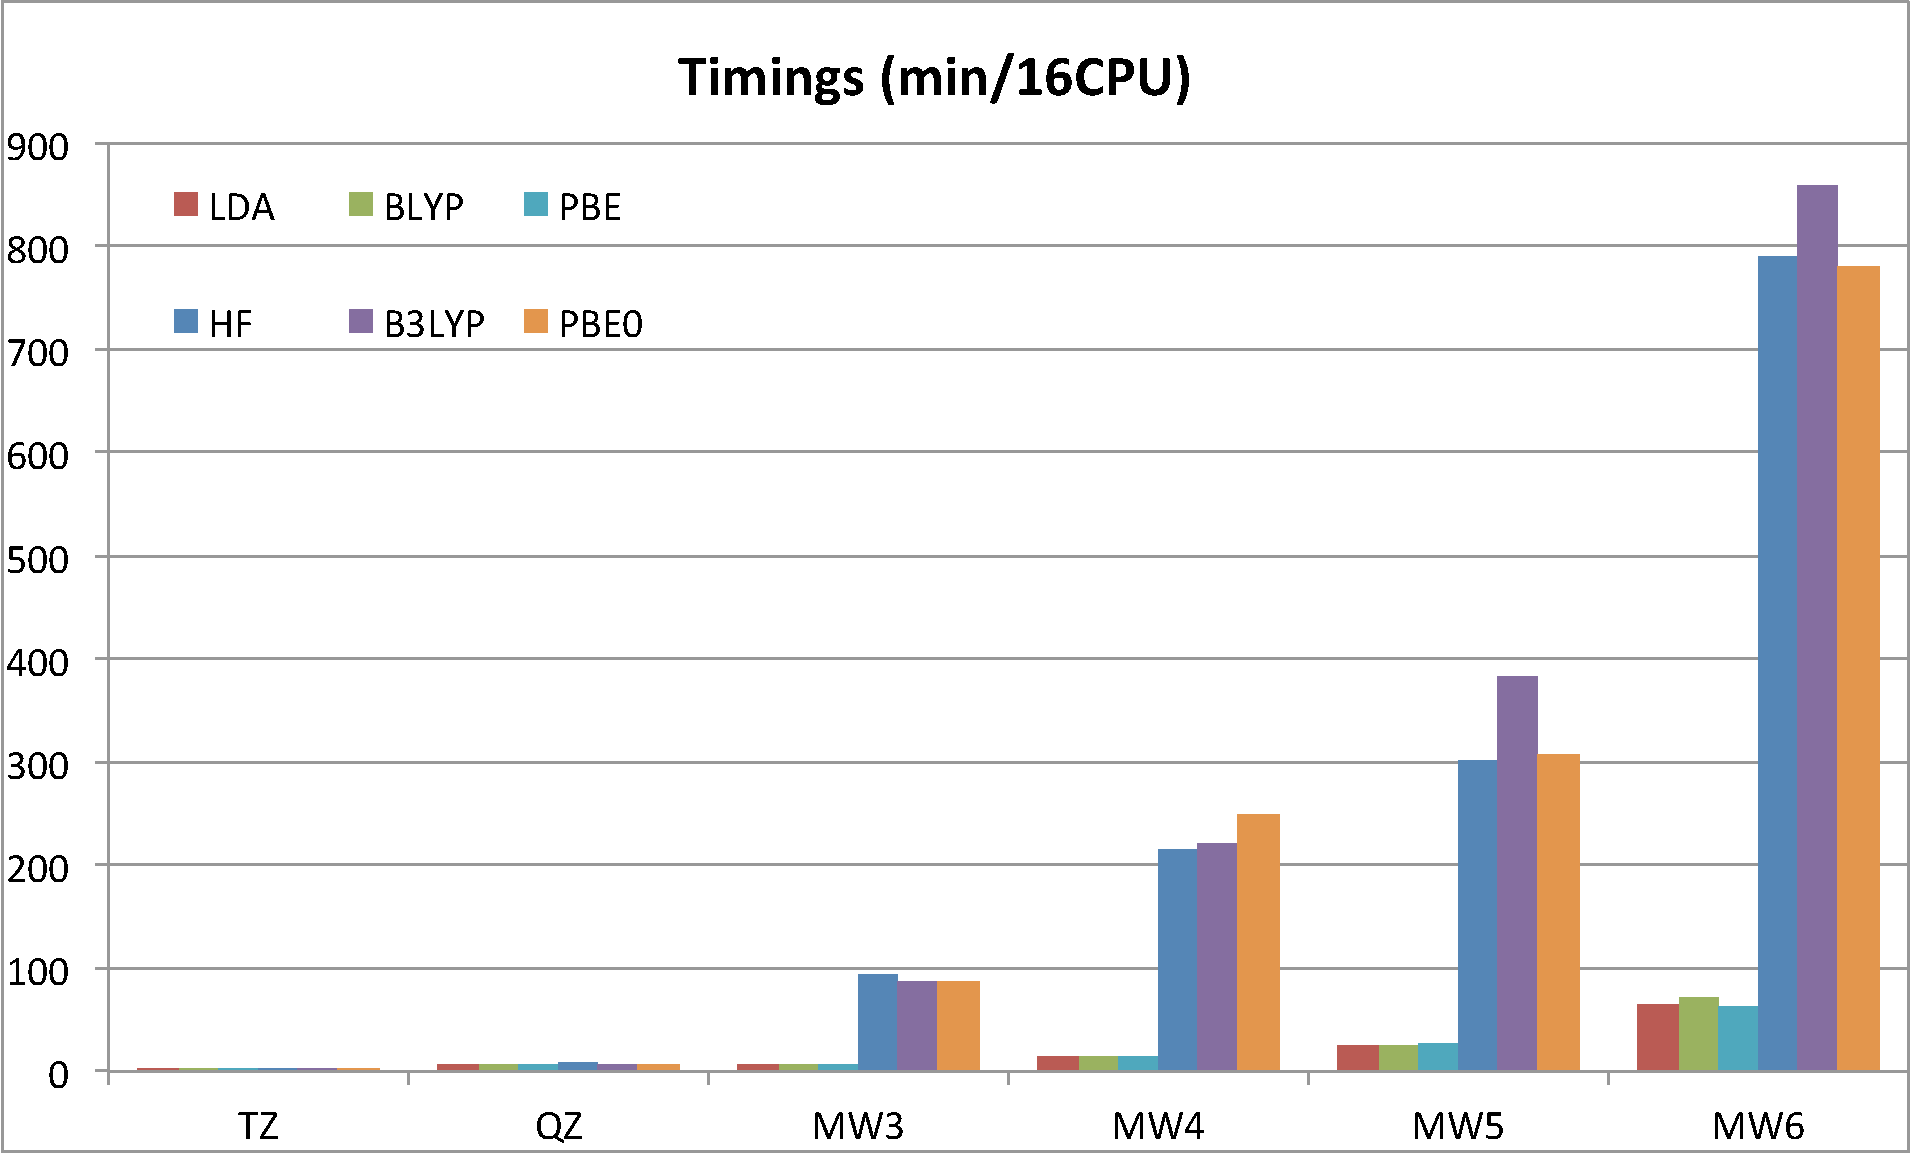
\includegraphics[scale=0.3]{figures/time_4.pdf}
\end{frame}

\begin{frame}
\frametitle{Comparison with Experiment}
\textbf{Calculations}
\begin{itemize}
    \item   MW calculations by MRChem
    \item   GTO calculations from Teale \etal
    \item   Basis sets: DZ, TZ, QZ, MW6
\end{itemize}

\vspace{10mm}

\textbf{Error analysis}
\begin{itemize}
    \item   NMR shielding constant (ppm)
    \item   1/4 of the data set excluded
    \item   Empirical equilibrium (experiments including ZPVC) is taken as reference
\end{itemize}
\end{frame}


\begin{frame}
\frametitle{Comparison with Experiment}
\centering
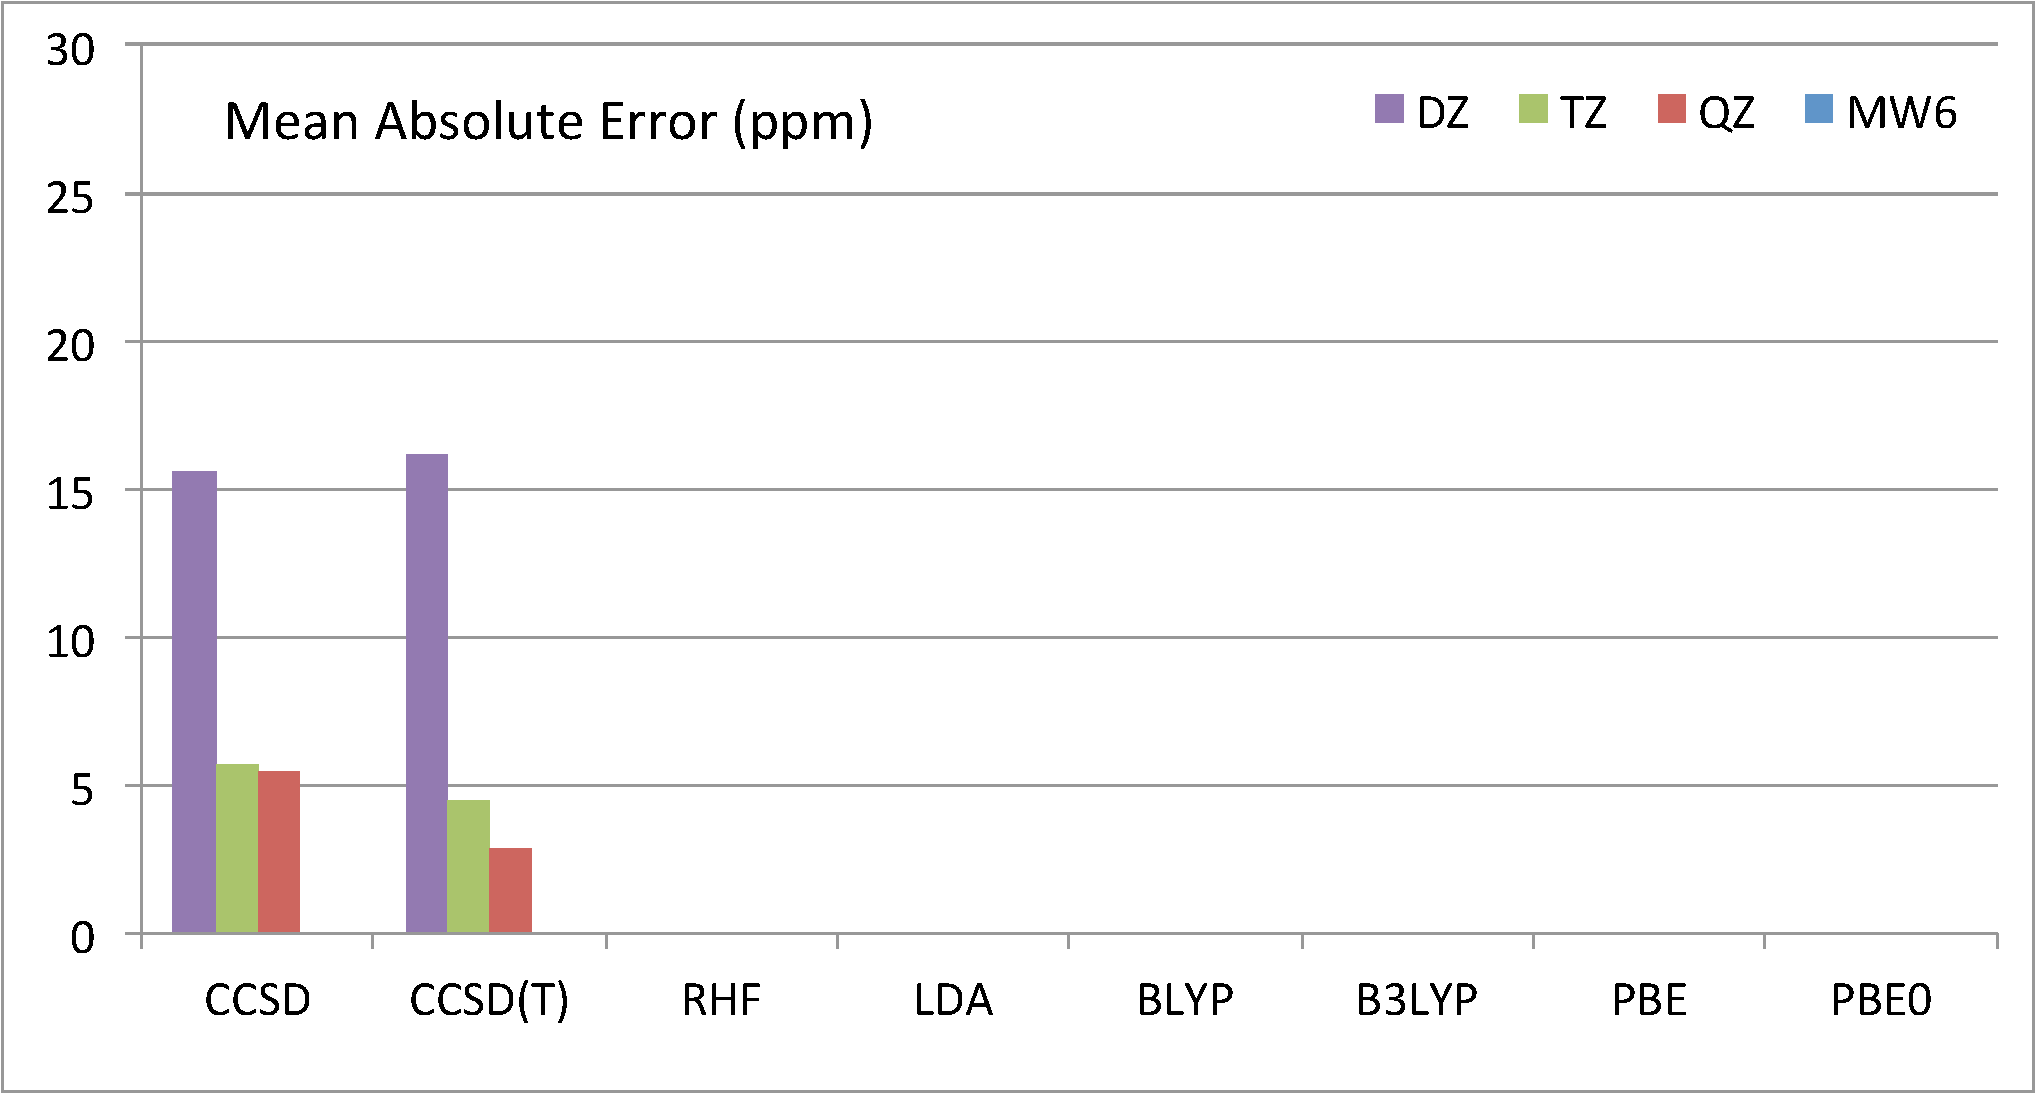
\includegraphics[scale=0.3]{figures/mae_exp_1.pdf}
\end{frame}

\begin{frame}
\frametitle{Comparison with Experiment}
\centering
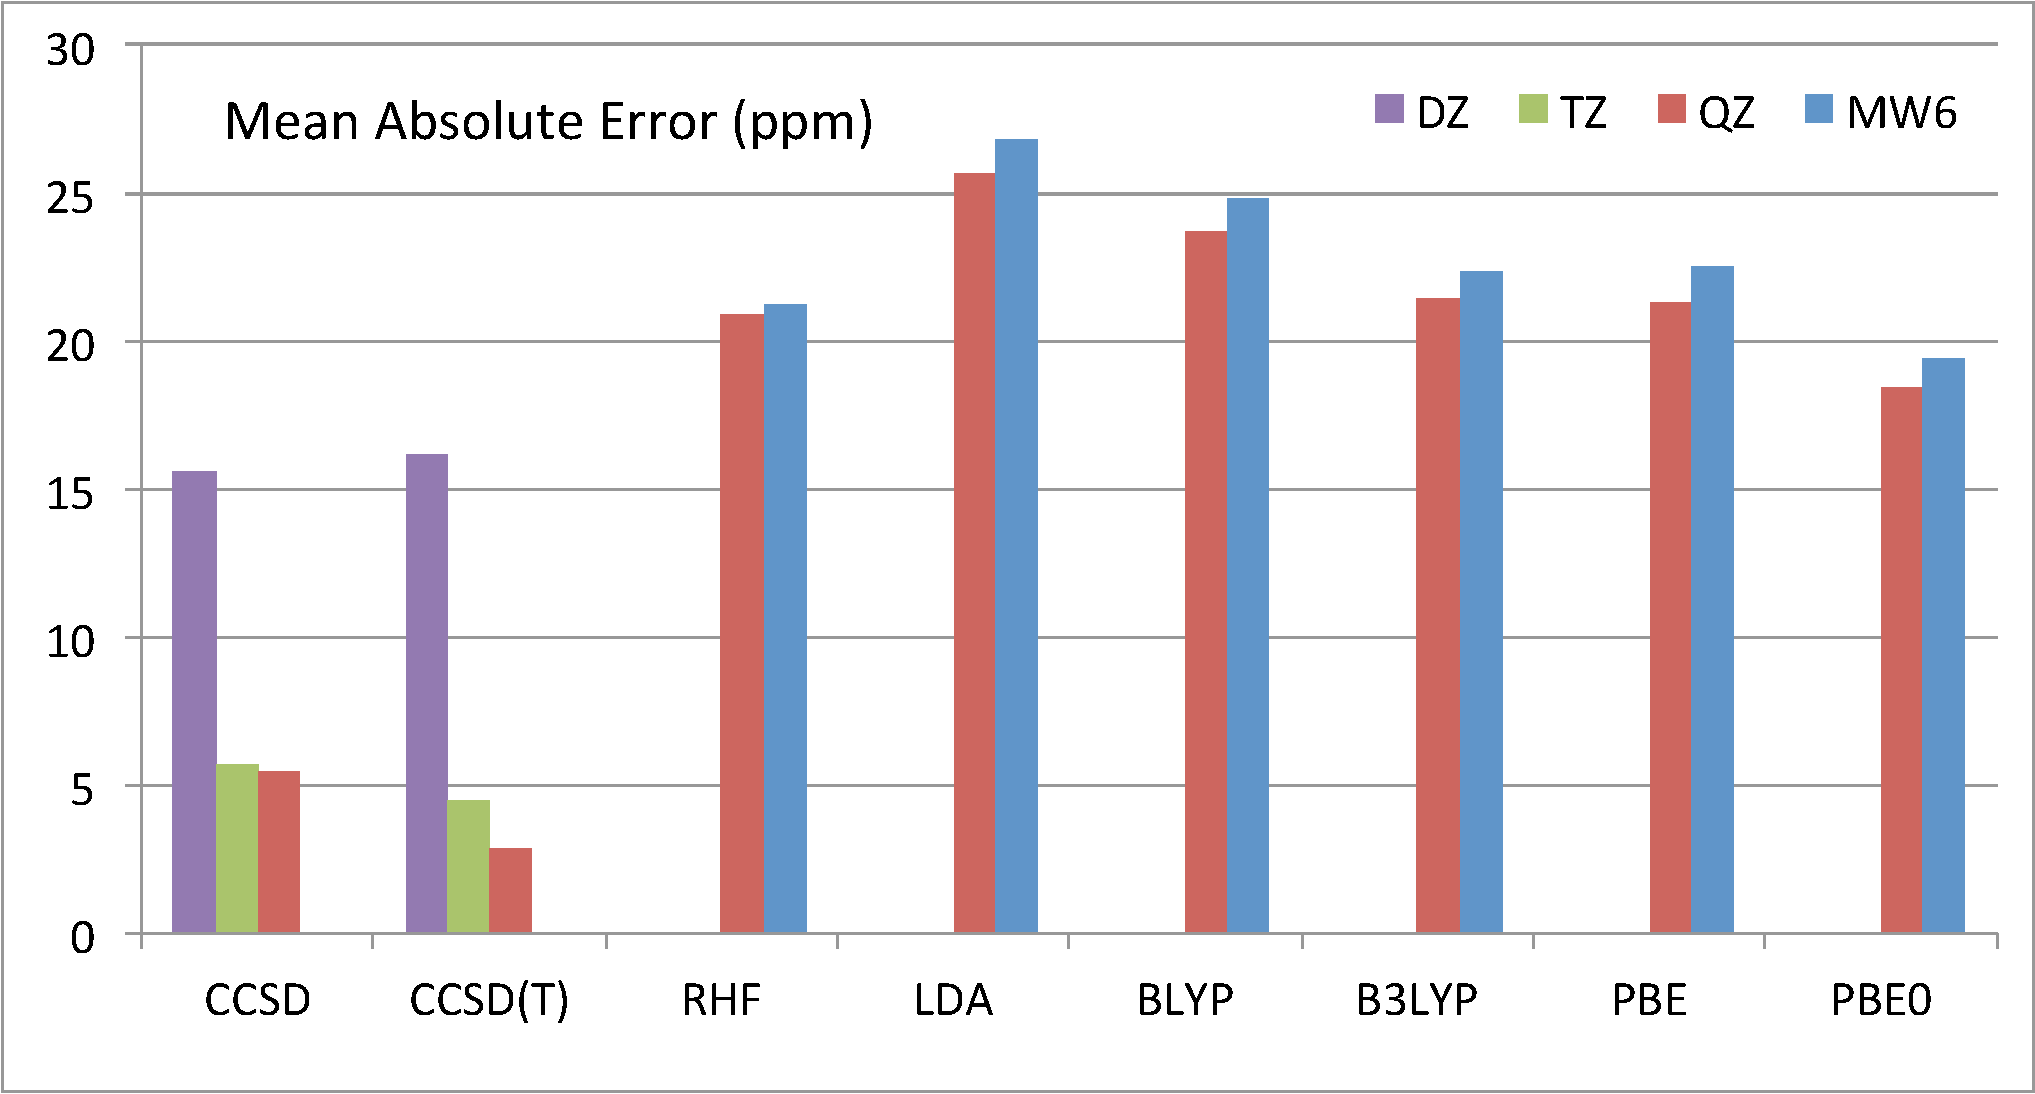
\includegraphics[scale=0.3]{figures/mae_exp_2.pdf}
\end{frame}

\begin{frame}
\frametitle{Comparison with Experiment}
\centering
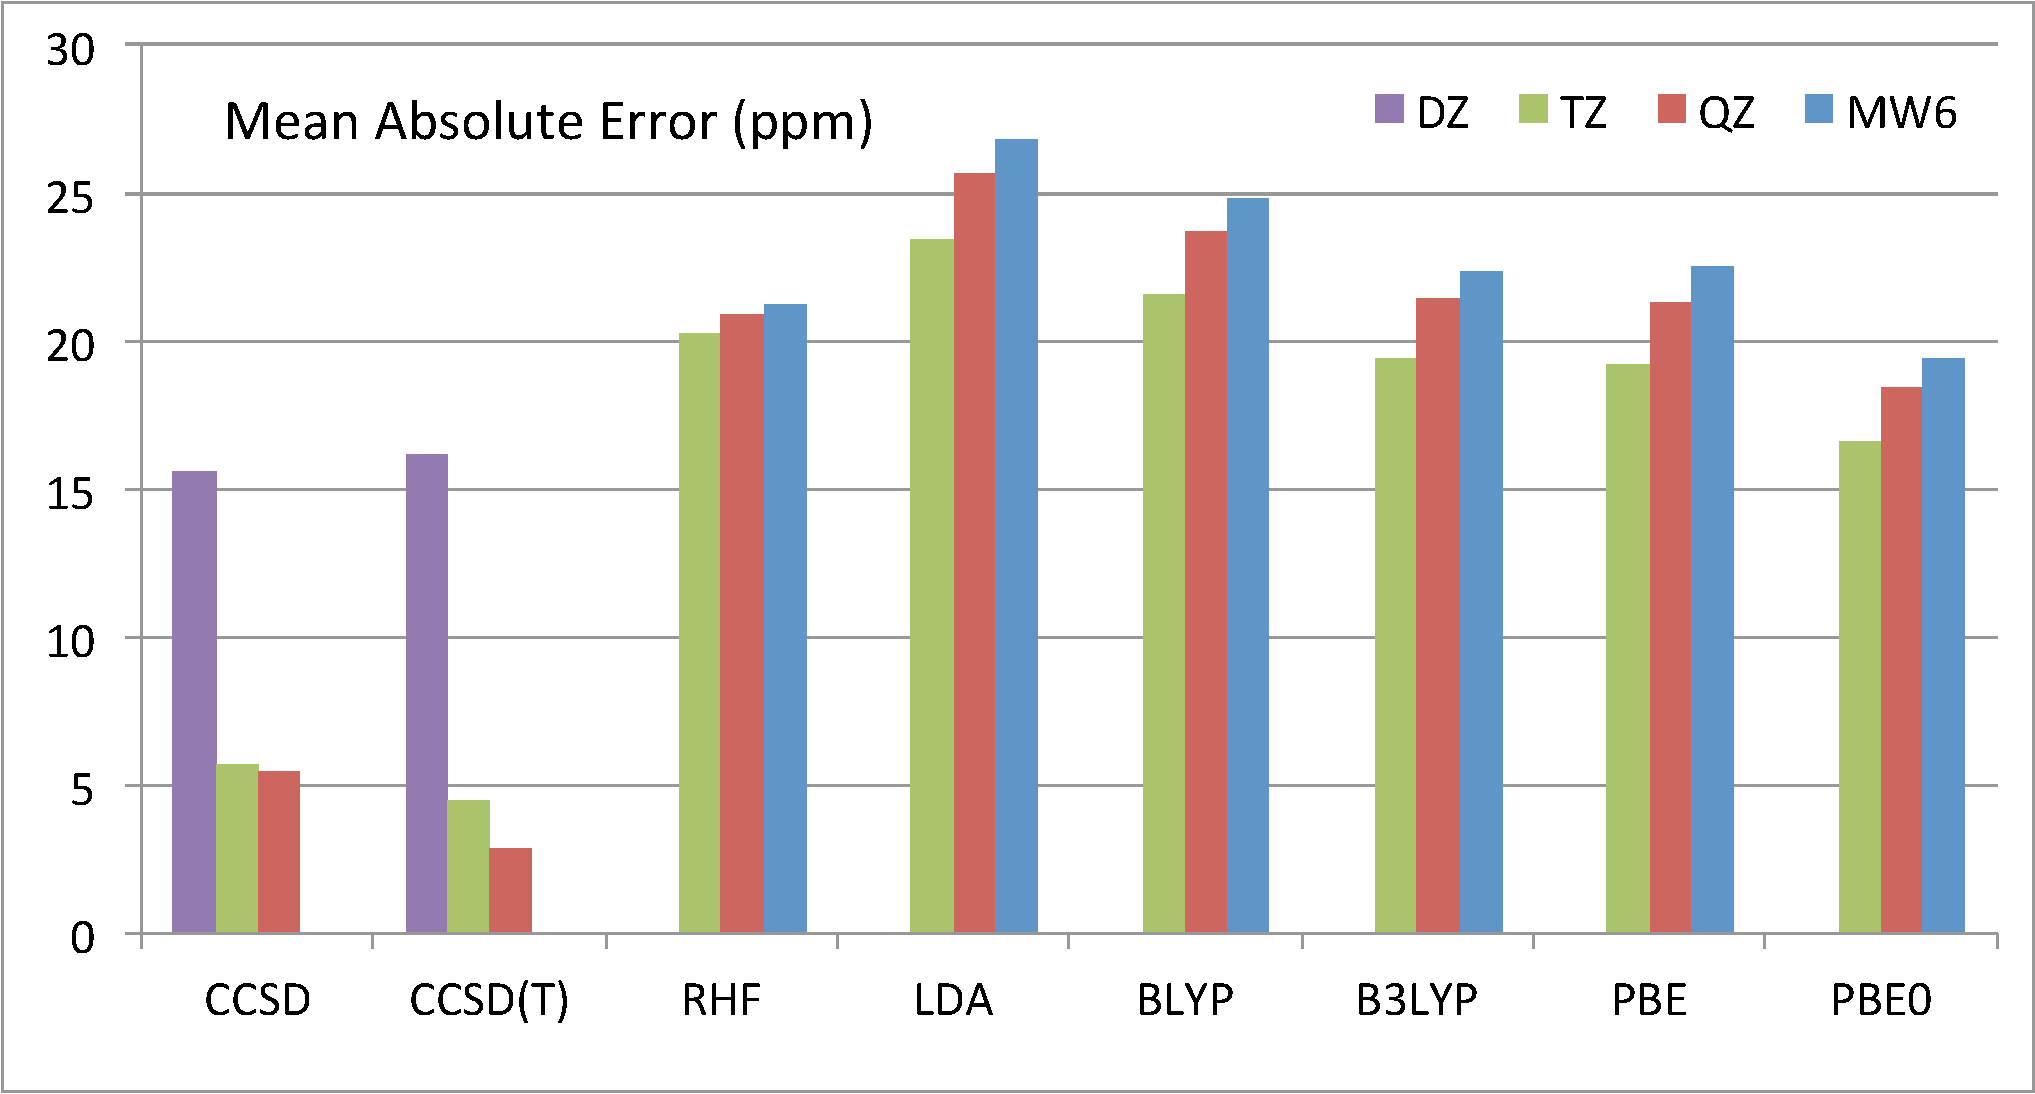
\includegraphics[scale=0.3]{figures/mae_exp_3.pdf}
\end{frame}

\begin{frame}
\frametitle{Comparison with Experiment}
\centering
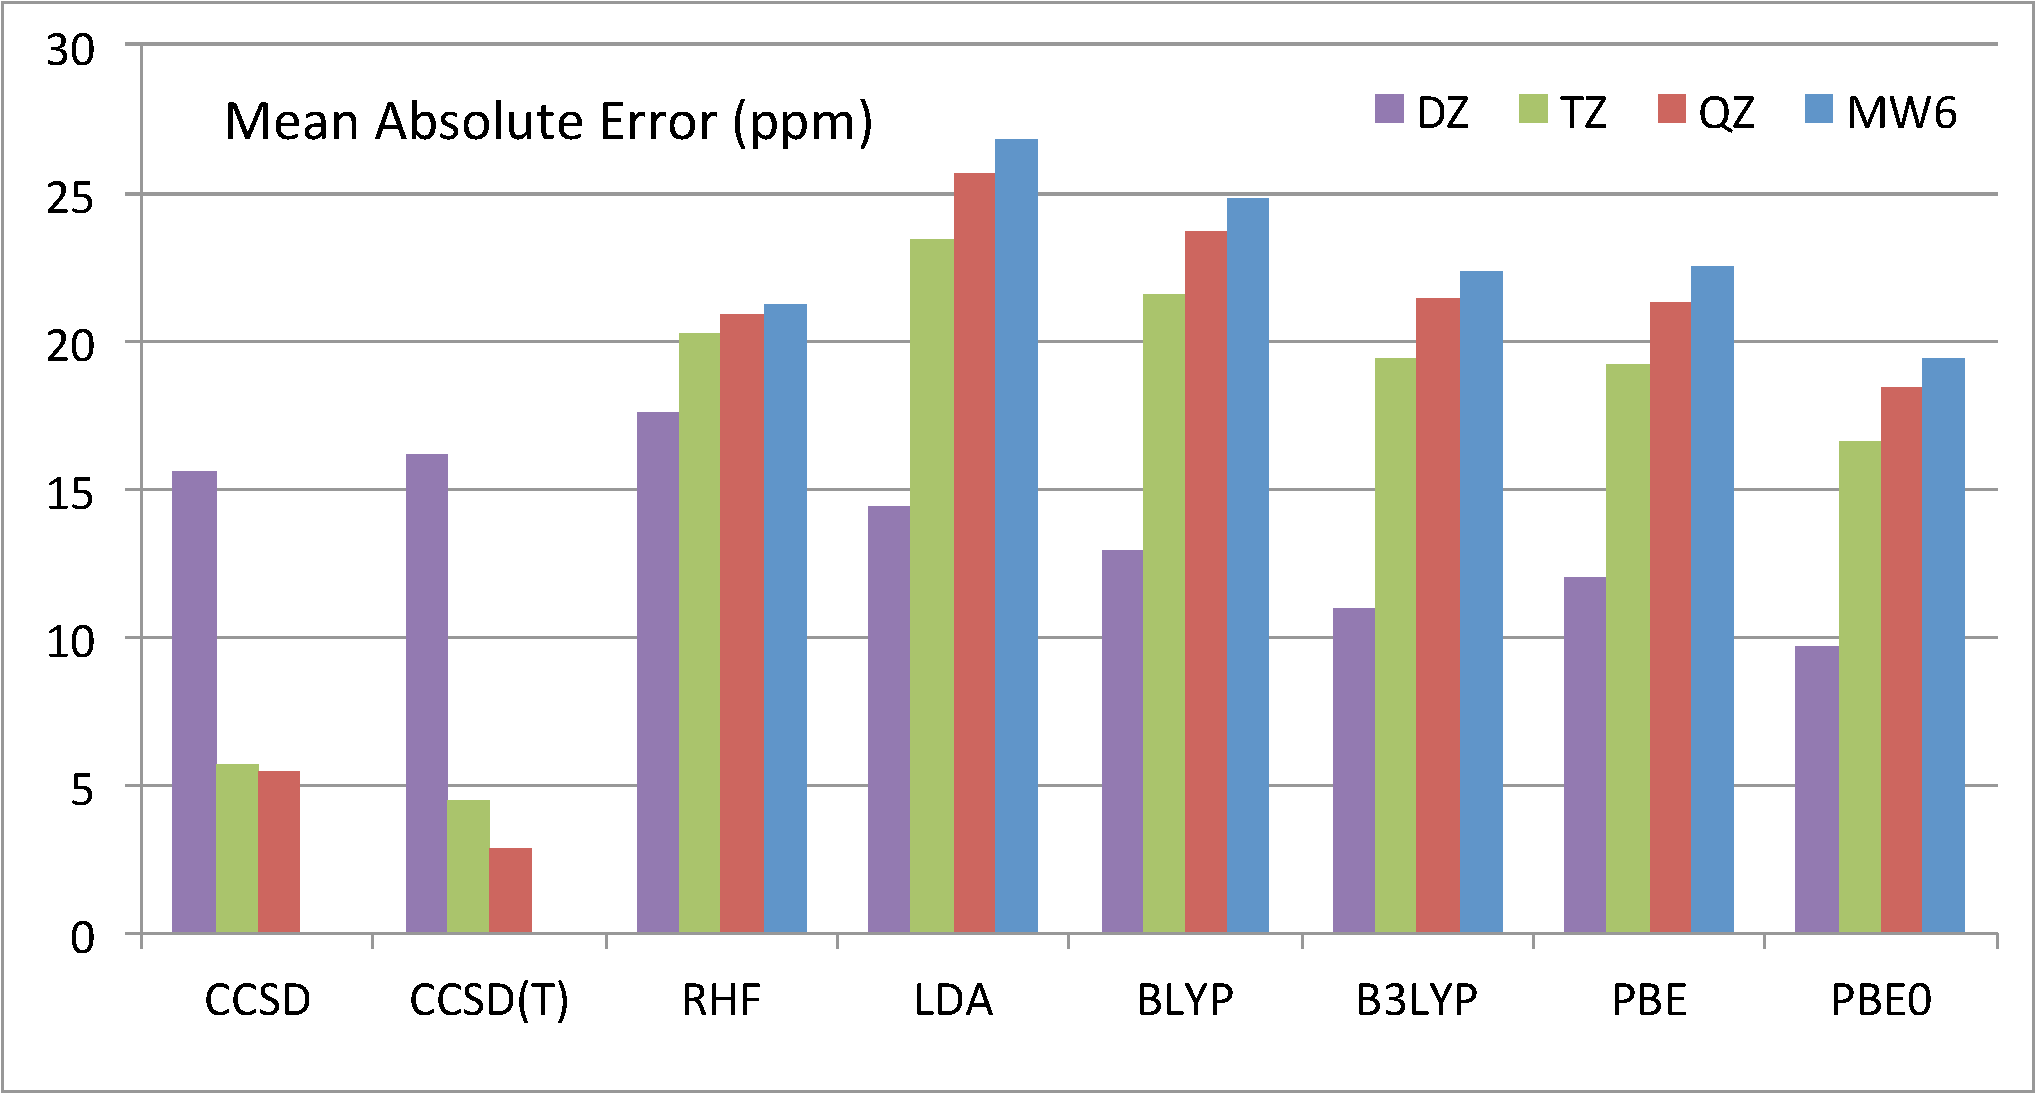
\includegraphics[scale=0.3]{figures/mae_exp_4.pdf}
\end{frame}


\end{document}
